\documentclass{lite}
\usepackage[
    letterpaper,
    tmargin=0.7in,
    lmargin=1.0in,
    rmargin=1.0in,
    bmargin=1.0in,
]{geometry}
\usepackage{caption}
% Page style
\usepackage{fancyhdr}
\usepackage[normalem]{ulem}
\usepackage{array}
\usepackage[inkscapelatex=false]{svg}

\pagestyle{fancy}
\fancyhead{}
\fancyfoot[C]{\thepage} % \fancyfoot{}
\setlength{\footskip}{45pt}
\renewcommand{\footrulewidth}{0pt}
\renewcommand{\headrulewidth}{0pt}


\def\jake#1{{\color{orange}$\mathtt{Jake:}$ {#1}}}


% bibliography
\addbibresource{refs.bib}
\AtBeginBibliography{\normalsize}

% new commands
\newcommand{\R}{\mathbb{R}}
\newcommand{\E}{\mathbb{E}}
\newcommand{\C}{\operatorname{Cov}}
\newcommand{\Cpsth}{\Sigma_{\text{PSTH}}}
\newcommand{\Cfem}{\Sigma_{\text{FEM}}}
\newcommand{\Ctotal}{\Sigma_{\text{total}}}
\newcommand{\Crate}{\Sigma_{\text{rate}}}
\newcommand{\ph}[1]{\textbf{[#1]}}

%%%%%%%%%%%%%%%%%%%%%%%%%%%%%%%%%%%%%%%%%%%%%%%%%%%%%
%%%%%%%%%%%%%%%%%%%%%%%%%%%%%%%%%%%%%%%%%%%%%%%%%%%%%

\begin{document}
\titlename{Active sensing explains cortical variability and improves visual information}{\today}

\begin{center}
\vspace{-0.25em}
{\large Ryan Ressmeyer$^{3*}$, Declan Rowley$^{4}$, Tejas Kothapalli$^{1,2*}$, Hadi Vafaii$^{1,2}$, Dekel Galor$^{1,2}$, Ruei-Jr Wu$^{5}$, Michele Rucci$^{5}$, Alexander C. Huk$^{4}$, Jude Mitchell$^{5}$, Daniel Butts$^{6}$, Jacob Yates$^{1,2}$\par}
% Include Gabe, Yonatan?
\vspace{0.35em}
{\small
$^{1}$ Redwood Center for Theoretical Neuroscience, UC Berkeley\\
$^{2}$ Herbert Wertheim School of Optometry and Vision Science, UC 
Berkeley\\
$^{3}$ University of Washington\\
$^{4}$ Fuster Laboratory for Cognitive Neuroscience, Departments of Psychiatry \& Biobehavioral Sciences and Ophthalmology, UCLA\\
$^{5}$ Brain and Cognitive Science, University of Rochester\\
$^{6}$ Department of Biology, University of Maryland, College Park\\
$^*$ Authors contributed equally
\par}
\vspace{1em}
\end{center}

% \date{\today}


\section{Introduction}
Vision is active, even during fixation. We have known for centuries that the eyes never rest \cite{Jurin1738, martinez2017unchanging}, and fixational eye movements (FEMs) continually translate the image across the retina. Decades of psychophysical work show that these minute displacements support fine spatial vision \cite{rucci2007miniature, ratnam2017benefits, intoy2020finely}. Theory explains how: retinal motion converts spatial structure into temporal signals that can improve visual encoding \cite{rucci2015unsteady, rucci2018temporal} and be utilized for hyperacuity \cite{anderson2020high}. Consistent with this account, neurophysiological studies have found substantial effects of FEMs in the retina \cite{wu2024fixational} and visual cortex \cite{baudot2013animation, mcfarland2016variability}. Yet how these movements shape visual encoding across cortical populations remains unknown.

How fixational eye movements (FEMs) influence visual encoding depends on the magnitude and structure of their effect on cortical population activity. Repeated presentations of the same stimulus are often assumed to be the same retinal input. But because gaze follows a different trajectory on each trial, repeated presentations do not repeat the same retinal input \cite{mcfarland2016variability}. The resulting differences in neural responses are ordinarily counted as internal variability \cite{shadlen1998variable} with consequences for coding that depend on structure of shared variability across the population \cite{averbeck2006neural, moreno2014information}. Independent fluctuations can be averaged across neurons, whereas shared fluctuations can enhance, impair or ultimately limit coding depending on their alignment with neuronal tuning. The amount of cortical activity driven by FEMs and how that activity is organized across the population remains unknown.

To distinguish between these possibilities, we characterized the structure of neural variability in the foveal region of marmoset visual cortex during alert fixation. We recorded simultaneously from populations of neurons using high-density silicon electrode arrays while tracking the subject's gaze with high-resolution eye tracking \cite{yates2023detailed, ressmeyer2025openirisdpi, wu2023high}. Using a principled decomposition based on the law of total covariance, we separated population variability into components attributable to stimulus-locked responses, fixational eye movements, and residual internal variability. 

FEMs accounted for most neural variability via feedback through reafference (i.e., through the retinal input). FEMs accounted for 70\% of the rate modulation in individual neurons, significantly more than the stimulus-locked average response. Traditional measures of variability were substantially reduced, and the structure of the variability induced by FEMs was low-dimensional and aligned with stimulus-driven population activity. Detailed analysis via a detailed simulation of the V1 population clarified that the trial-by-trial variability during fixation was primarily explained by changes in the retinal input, revealing a reafferent eye-brain-environment feedback loop.


Visual information was increased by FEMs in select neural subpopulations, depending on the metrics of the eye movement and the stimulus content. Real FEMs produced more informative activations than counterfactually stabilized input. Further, the size of the FEMs interacted with both the tuning of the neurons and the stimulus content to increase stimulus information dynamically as a function of the gaze trajectory. Taken together, these results reveal the structure, mechanism and function of FEM modulation in foveal V1.


% We move our eyes to see \cite{steinman1996moveo}. In primates, a small patch of retina, the fovea, carries the bulk of high acuity vision \cite{grunert2021morphology} and gaze shifts are the mechanism that position this patch over features of interest \cite{gibson2014ecological}. Yet even when gaze is held still, the eyes do not stop \cite{rucci2015unsteady}. During fixation they drift, tremble, and flick \cite{rucci2015control}, motions already evident in the earliest eye movement recordings \cite{adler1934influence}.

% For roughly a century, there has been an active debate about the significance of fixational movements \cite{steinman1996moveo}. One view treated them as motor noise, an unavoidable imperfection in the oculomotor system \cite{barlow1952eye}. Another proposed that they play a functional role in vision \cite{riggs1951visual}. More recently, experiments have demonstrated that fixational motion redistributes spatial information over time in ways that benefit perception \cite{rucci2007miniature, rucci2015unsteady, intoy2020finely}. Despite this long history, it remains unresolved whether these movements are an essential component of the neural code during normal vision.

% A parallel debate revolves around the shared variability in visual cortical neurons \cite{kohn2016correlations}. Neurons in visual cortex are notoriously variable, even under carefully controlled conditions \cite{tolhurst1983statistical}. This variability is not independent across neurons but shared and structured at the population level \cite{arieli1996dynamics, kenet2003spontaneously}. It has been quantified using measures such as Fano factors \cite{churchland2010stimulus}, noise correlations \cite{cohen2011measuring}, and low-dimensional latent variable models \cite{ecker2014state, zhao2020stimulus}, and is interpreted as stochastic spiking noise \cite{pouget2000information}, fluctuations in internal state \cite{ecker2014state}, or ongoing cortical dynamics \cite{arieli1996dynamics, kenet2003spontaneously, stringer2019spontaneous}. Whether or not this variability is ``noise'' or essential signal remains unknown.

% Variability in cortex is widely assumed to be internal to the brain, even when linked to externally measured behavior \cite{stringer2019spontaneous, kang2025impact}; yet, they could be the result of active sensing strategies \cite{rucci2018temporal, gruber2021oculo, ahissar2025closed}. In support of this, previous work has shown that individual neurons in V1 respond more precisely to stimuli jittered by fixational eye movements \cite{baudot2013animation}, are precise once accounting for retinal position \cite{gur2006high}, and have substantial variability attributable to fixational eye movements \cite{mcfarland2016variability}.

% To distinguish between these possibilities, we
% characterized the structure of neural variability in the foveal region of marmoset visual cortex during alert fixation. We
% recorded simultaneously from populations of neurons using high-density silicon electrode arrays while tracking the subject's gaze with high-resolution eye tracking \cite{yates2023detailed, ressmeyer2025openirisdpi, wu2023high}. Using a principled decomposition based on the law of total covariance, we separated population variability into components attributable to stimulus-locked responses, fixational eye movements, and residual internal variability. This framework allowed us to assess how much shared variability can be explained by measured retinal motion, and how this variability is structured across neural populations.

% To relate variability structure to visual function, we further employed an image-computable population model trained to predict neural responses during free viewing \cite{yates2023detailed}. This model enabled us to quantify how eye-movement–dependent modulations of retinal input shape trial-by-trial population responses and visual information. Together, these analyses support a unified view in which fixational eye movements are a dominant and structured component of active sensing in foveal visual cortex. Rather than reflecting substantial internal neural noise, shared population variability largely captures systematic, behaviorally generated modulation of retinal input that is structured along stimulus-tuned dimensions and enhances spatial information.

\section{Results}

%\subsection{Population recordings during foveal fixation reveal structured trial-by-trial variability}
\subsection{Small fixational eye movements exert large effects on the structure of neural responses}

We recorded from populations of 13-132 units in the foveal representation of primary visual cortex (V1) in 2 awake marmosets. Subjects maintained stable fixation within a 1° window while viewing a repeated sequence of rapidly flashed, whitened natural images presented at 20 Hz (Fig. 1A). Gaze position was monitored using high-resolution eye tracking \cite{yates2023detailed} and remained well within the fixation window across trials (Fig. 1B). These fixation distributions are similar to those observed in humans and macaques \cite{cherici2012precision, ressmeyer2025openirisdpi}. Receptive fields of recorded units were confined to eccentricities of $<$1° (Fig. 1C). As expected, activity was elicited in the recorded units by the visual stimuli presented over their receptive fields (RF), and the resulting patterns of spikes were variable from trial to trial (Fig. 1D). 

To visualize whether conditioning on gaze position revealed structure in the cross-trial variability, we isolated the relative displacement of the eye between trials across the feature tuning of individual units (Fig. 1E, extended data figure 1) and show that ordering the stimulus evoked responses by these small gaze displacements reveals striking structure in the trial-to-trial fluctuations (Fig. 1F). Indeed, comparing the average response from trials split by relative eye position (Fig. 1G) reveals markedly different timecourses of activity, providing evidence that FEMs can substantially structure neural activity in individual neurons.

Response structuring by FEMs was evident at the population level as well. We visualized population level rasters from multiple trials while conditioning on clusters of similar gaze trajectories. We identified two groups of trials with highly self-similar eye trajectories, but which differed from one other (Fig. 1H). Population responses were reproducible within each group (trials 1-4, blue), whereas trials with distinct trajectories exhibited systematically different patterns of activity (trials 5-8, red; Fig. 1I). These distinct profiles are apparent in the group-averaged population responses (Fig. 1J)-- even though the stimulus was identical across all trials. 

These visualizations suggest that FEMs structure responses at both the single-trial/single-neuron and ensemble levels. A major limitation of conditioning on gaze position in this manner is that very few, if any, trials result where the gaze trajectories are identical, resulting in a massive reduction in statistical power. We therefore leveraged a statistical approach to rigorously quantify how FEMs modulate population co-variability and shape the neural code for high precision vision \cite{mcfarland2016variability}. 

%% START OLD TEXT (RAR replaced 6/28/26)
%We recorded from populations of XX-XX neurons in the foveal representation of primary visual cortex (V1) in 2 alert marmosets. Subjects maintained stable fixation within a 1° window while viewing a repeated sequence of rapidly flashed, whitened natural images presented at 20 Hz (Fig. 1A). Fixation behavior was stable within and across trials (Fig. 1B), and contained small fixational eye movements similar to those observed in humans and macaques \cite{cherici2012precision, ressmeyer2025openirisdpi}. Receptive fields of recorded units were confined to eccentricities of $<$ 1° (Fig. 1C). %Single-trial population activity aligned to stimulus onset revealed coordinated fluctuations in firing across the population within individual trials (Fig. 1i), suggesting substantial shared variability beyond stimulus-locked responses.

%As expected, activity in these neurons was elicited by visual stimuli within the receptive field (RF) and was highly variable from trial to trial (Fig. 1D; citations). To examine whether this variability was related to fixational eye movements, we inspected both activity in light of measured FEMs on each trial. Reordering the trials to reflect the exact position of the gaze relative to the RF during stimulus viewing (Fig. 1E) revealed clusters of similar spike trains (Fig. 1F). Sorting the responses into two groups reflecting fixations to the left and right of the center of the receptive field resulted in two very different peri-stimulus time histograms, providing visual confirmation that FEMs matter (Fig. 1G). 

%Similar structuring by FEMs was visually evident in the shared variability across the population. We identified groups of trials and times with highly similar eye trajectories (Fig. 1H) and compared population responses across these groups. Within each group, population activity patterns were reproducible across trials (Fig 1I), whereas responses differed systematically between groups with distinct eye trajectories (Fig. 1J). This suggests that a large fraction of trial-to-trial population variability is the result of eye movements.
%% END OLD TEXT (RAR replaced 6/28/26)

% OLD text, clipped for now: ... sharpened substantially, revealing fine temporal structure that was obscured in the stimulus-aligned view (Fig. 1i). Together, these results indicate that fixational eye movements impose a structured, population-wide signature on neural activity.we compared population responses before and after conditioning on eye position.

% To quantify this organization, we tested whether eye state could be decoded directly from population activity on single trials. A linear decoder trained to predict discretized eye position from population spike counts performed significantly above chance (XX[XX,XX] \%; chance = XX \%), even after subtracting stimulus-locked activity. Decoding performance collapsed to chance when eye trajectories were permuted across trials, confirming that decoding relied on trial-specific coupling between eye movements and population activity (Fig. 1j). 


\begin{figure}[p]
    \centering
 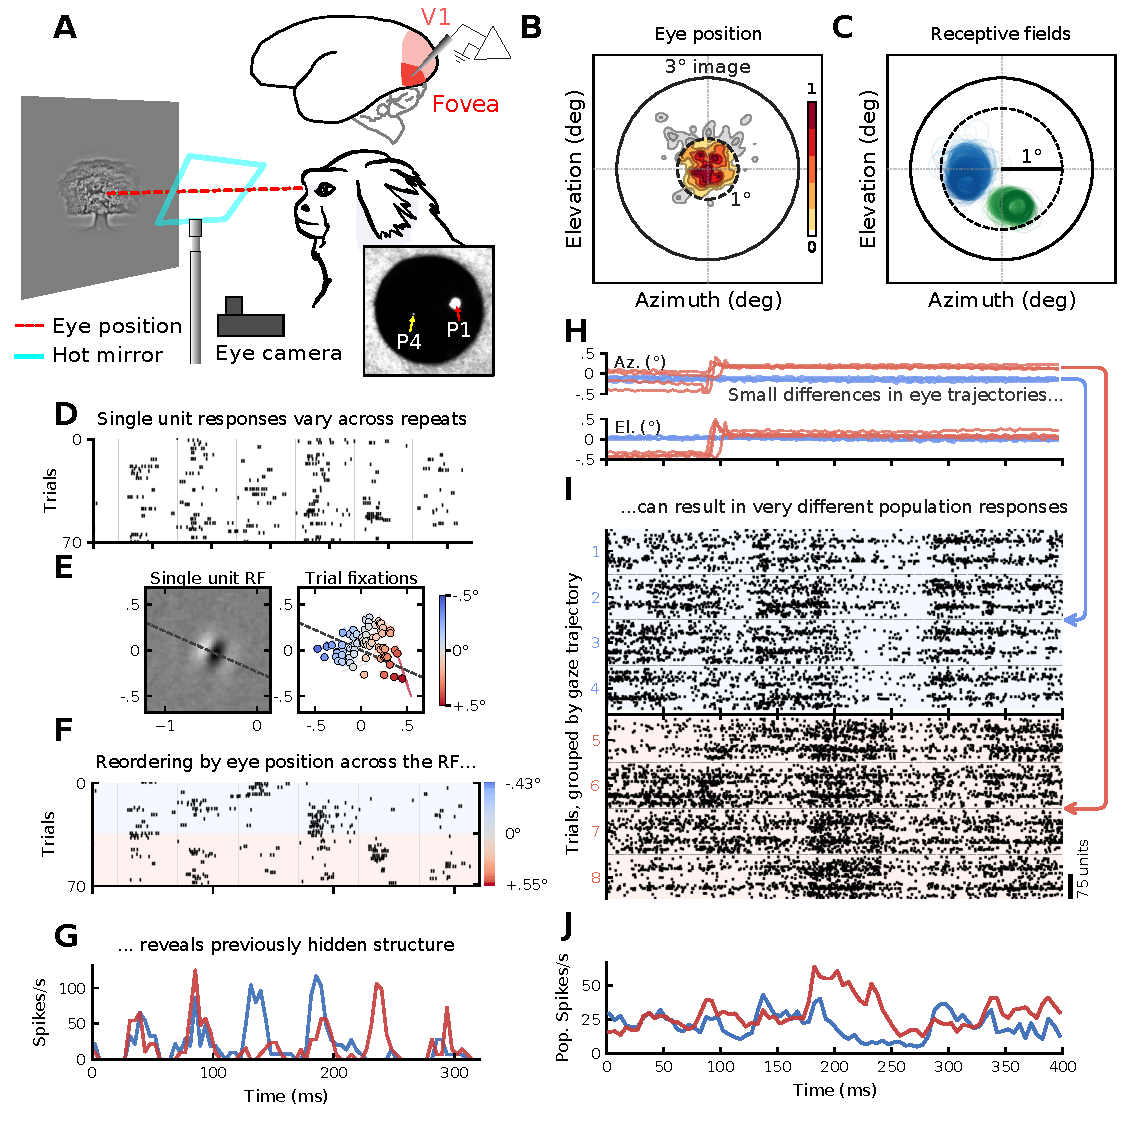
\includegraphics[width=\columnwidth, height=0.9 \textheight,keepaspectratio]{figures/figure1.pdf} 
     \caption{
     \textbf{Small eye movements structure neural activity within the foveal representation in primary visual cortex} 
    \textbf{(A)} Schematic of the experimental paradigm. A head-fixed marmoset fixated a rapidly updating sequence of flashed images ($3^\circ$ diameter). Electrical activity was recorded using laminar probes from the lateral surface of V1. The eye's position was tracked using a high-precision digital dual Purkinje image eye tracker. The eye was imaged through a hot mirror that allowed the subject to view the stimulus. A representative image of the Purkinje images is shown in the inset.
    \textbf{(B)} Distribution of eye positions during fixation for a representative experiment. Marmosets maintained tight fixational control, which was further refined by only considering eye positions within a $1^\circ$ diameter circle for analysis.
    \textbf{(C)} Receptive field (RF) locations. The extent of each unit's RF is drawn as a contour. Blue contours represent units recorded from monkey A, and green contours from monkey L. All units had receptive fields within $1^\circ$ from the fovea.} % Optional marker
    \label{fig:fig1}
\end{figure}

%\clearpage

\begin{figure}[p]
    \ContinuedFloat
    \caption[]{
    \textbf{(D)} Trial rasters for an the example unit, ordered by trial number. The single-unit responses vary across repeated stimulus presentations. 
    \textbf{(E)} Left: The RF for the unit shown in (D), which was obtained by spike-triggered averaging. The RF displays clear, Gabor-like structure. Right: The average eye position in a 50 ms bin across trials. Points are colored according to their projection onto the line orthogonal to the subunits of the RF. 
    \textbf{(F)} Trial rasters sorted by eye position across the RF. Sorting is performed independently for each 50 ms. Smooth variation in trial-to-trial responses emerges when sorting by eye position, indicating a relation between the eye's position and the neural response. 
    \textbf{(G)} The peristimulus time histogram of responses with positive projections across the RF (blue) and negative projections (red). Average stimulus-evoked responses diverge strongly between 100 ms and 250 ms. 
    \textbf{(H)}  Eye position over time for eight representative trials colored in red and blue. The eye position traces are highly self-similar within groups, but not between groups. 
    \textbf{(I)} Population rasters for the eight representative trials from (H). There is clear similarity between population responses on trials with similar eye trajectories, and large differences between trials with dissimilar eye trajectory, despite the fact that the difference in position is just fractions of a degree. 
    \textbf{(J)} Spiking activity averaged across all recorded units for the four red trials and four blue trials over the same time course. The average population firing rate diverges strongly around 200 ms in the trial. 
    }
\end{figure}

\clearpage

% \begin{figure}[h!]
%     \centering
%     
\includegraphics[width=\linewidth]{figures/fig1.pdf}
%      \caption*{
%      \textbf{Small fixational eye movements exert large effects on the structure of neural variability.}
%     \textbf{(A)} Schematic of the experimental approach. A head fixed marmoset fixated a sequence of rapidly flashed images. Neural activity was recorded from the lateral surface of V1, corresponding to the foveal representation. 
%     \textbf{(B)} The distribution of gaze during an example experiments shows tight oculomotor control by the marmosets. A majority of gaze positions were within 0.5 deg during the experiment. } % Optional marker
% \end{figure}

% \clearpage % Forces the next content to a new page

% \begin{figure}[t]
%     \ContinuedFloat
%     \caption{
%     \textbf{(C)} Receptive field locations for each experiment. Blue represents RFs of units recorded from monkey A, while green represents RFs from monkey L. 
%     \textbf{(D)} Left: An example STA for a single foveal unit with clear gabor-like structure. A line denoting the orthogonal direction to the subunits is drawn to indicate the direction with maximal sensitivity to changes in position under a linear model of the unit's response. Right: The position of gaze measured across all trials in a 50ms bin. Points are colored according to their projection on to the line of maximal sensitivity determined in the left plot. 
%     \textbf{(E)} The peristimulus time histogram of responses for the example unit shown in (D). The gray trace depicts the overall PSTH across all trials, while the blue and red lines represent the PSTH of the trials with positive or negative or negative projections onto the line of maximum sensitivity. Since eye position is not steady throughout individual trials, the projection is computed on the average gaze position in 50 ms bins. 
%     \textbf{(F)} Trial rasters sorted by the position of gaze projected onto the line of maximum sensitivity. Sorting occurs on the same bins as in (E). Clear structure emerges when sorting by eye position. 
%     \textbf{(G)} Gaze position over time for eight representative trials colored in red and blue. The eye position traces are highly self similar within groups (between blue traces, for example), but not between groups (between red and blue traces). 
%     \textbf{(H)} Spiking activity averaged across all recorded units for the four red trials (red) and four blue trials (blue) over the same time course. 
%     \textbf{(I)} Population rasters for the eight representative trials from (H) and (I). There is clear similarity between individual trials with similar gaze traces, and large differences at the population level between trials with dissimilar gaze, even though the difference in position is just fractions of a degree.} 
%     \label{fig:fig1}
% \end{figure}


\subsection{Active sensing accounts for most residual neural variability}

To quantify the contribution of FEMs to neural variability, we extended and applied a recently developed method for neural variability decomposition (\cite{mcfarland2016variability}; methods). This approach relies on the fact that the same time-varying visual stimulus is present on each trial, but the eye position is variable. By considering the similarity of the eye trajectories leading up to a given timepoint (Fig. 2A), the distance between the trajectories dictates whether the spikes from two trials (at that time bin) come from the same stimulus or a different stimulus. This analysis can separate intrinsic variability (present across trials even when eye position is identical) from FEM-driven variability (which will be dependent on the degree of FEM dissimilarity across trials).

%By matching pairs of timepoints across trials based on the similarity of the eye trajectory leading up to that timepoint, it uses these pairs to compute the reliable variance given consistent retinal input (Fig 2A). Trials with similar eye position trajectories 
%This formalizes the intuition that when the eye position is similar across trials, then the neural response is expected to be similar;  when the eye position is different, then the neural response is expected to be different. 

%The method allowed us to quantify the amount of consistent variability in the neural responses given at most a set level of eye-position similarity between trials. In the limit of a completely permissive threshold, this measure simply recapitulates the total variance in the average response across trials (i.e., the peri-stimulus time histogram, or PSTH, variance; \cite{sahani2003linear}). However, as the requirement on eye-position similarity is made more stringent the amount of consistent variance across trials increases, indicating that a substantial fraction of the trial-to-trial variability in neural responses is attributable to differences in eye position (Fig 2B). 
Following this logic, we found that the variability left unaccounted-for when eye trajectories were highly mismatched comprised most of the total variability, meaning that the stimulus alone accounted for only a fraction of the total variability (Fig 2B, red). However, for eye trajectories that were more similar, variability that remained unaccounted-for dropped considerably (Fig 2B, blue). 
%We then quantified the extent to which conditioning on nearly identical eye position trajectories ($\Delta e < 0.05^\circ$) recovered reliable variation in single-neuron responses, computing the fraction of total reliable variance recovered by accounting for FEMs. 
We then quantified the fraction of total accountable variance attributable to FEMs. Across the population, the majority of the rate variance of individual units was explained by FEMs, with a median of $0.71$ (IQR $[0.57, 0.81]$; trajectory-shuffle test $p = 0.007$; Fig.~2C). This suggests that the neural responses in our foveal recordings were driven more by the trial-by-trial differences in gaze trajectory than by the stimulus changes, which is striking given that the fixation behavior was very stable by conventional standards. 

We then applied this decomposition approach to quantify the contribution of FEMs to shared variability across neural population. 
%Classical studies decompose the joint variability of simultaneously recorded neurons into a stimulus-driven component and a residual (noise) component by referencing each trial to the trial-averaged response (\cite{bair2001correlated,kohn2005stimulus}). However, this approach does not account for the fact that FEMs can drive shared variability across neurons. Using the law of total covariance, 
We decomposed the total covariance into three components: stimulus-locked covariance ($\Cpsth$), eye-movement--dependent rate covariance ($\Cfem$), and residual internal covariance ($\Sigma_{\text{int}}$; Fig 2D). This decomposition revealed that substantial shared variability was attributable to FEMs. This was apparent in the population Fano factor
% -- the slope of the variance-to-mean relationship across neurons within a recording \cite{churchland2010stimulus}-- 
which decreased substantially when taking FEMs into account, from $1.24$ to the sub-Poisson value of $0.80$ (a reduction absent under the trajectory shuffle, empirical $p<0.001$; Fig.~2E). Further, estimates of shared variability across neurons (``noise correlations") also decreased significantly, from levels comparable to other reports ($\rho = 0.077$ [$0.067$, $0.088$]; citations) to a level statistically indistinguishable from zero ($\rho = 0.010$ [$-0.009$, $0.030$]; $\Delta \rho = -0.067$ [$-0.086$, $-0.050$] vs.\ a shuffle null of $[-0.011, 0.011]$, empirical $p<0.001$). These results demonstrate that neurons in foveal V1 are less intrinsically variable than typically thought, and that the majority of shared variability not captured by the average response over trials can be attributed to differences in eye position across trials. In short, once one factors out the effects of tiny FEMs, foveal V1 neurons are individually rather precise, and are collectively uncorrelated. 

FEM-induced variability was not only a large portion of the shared variability, but also strongly structured. The FEM-driven covariance was low-dimensional (participation ratio $3.4 \pm 1.2$, averaged across sessions), roughly seven-fold more compact than the residual covariance that remained ($24.4 \pm 14.8$), and indistinguishable from the dimensionality of the stimulus-driven covariance $\Cpsth$ ($3.6 \pm 1.0$; Fig. 2G). 

The compactness of $\Cfem$ raises a sharper question: do fixational eye movements drive activity along the same population dimensions that encode the stimulus, or along orthogonal ones? There is good reason to expect the former. A neuron responds to the image on its receptive field, and the eye moving across the image changes that image much as the stimulus changing does. Both should therefore drive the population along the same dimensions. From a classic population coding perspective, such variability is the worst case: it looks like a change in the stimulus, so averaging over more neurons does not remove it [14]. But if it is driven by FEMs, it looks like a stimulus change because the retinal image did change, and what is information-limiting correlation for a decoder blind to eye position is in fact signal for one that is not.

We addressed this question by measuring how well the leading subspace of one covariance component captured the variance of the other, projecting each component onto the leading eigenvectors of its counterpart and computing the fraction of variance retained. A value near one is achieved when the two share a subspace and near zero when they are orthogonal (Fig. 2H; methods). Because both components are low-dimensional, we tested this alignment in both directions and against a shuffle null that destroyed the trial-specific coupling between eye position and population activity. The two subspaces showed alignment far above chance: a majority of the stimulus-driven variance fell within the FEM subspace ($0.60 \pm 0.11$), and, symmetrically, a majority of the FEM-driven variance fell within the stimulus subspace ($0.63 \pm 0.14$), each well above its shuffle null ($\approx 0.35$; $p < 0.001$ for both directions; Fig. 2I). FEM-driven modulation is therefore largely confined to the same low-dimensional subspace that carries the population's stimulus response \cite{liska2024running}. For a decoder with no access to eye position, this is the geometry of an information-limiting correlation \cite{moreno2014information}: this is a worse-case scenario for trial-to-trial variability, as it is indistinguishable from a true change in the stimulus. However, for a decoder that has access to eye position, the same component becomes a recoverable signal given the position of the eye. We therefore investigated how the brain might make use of an FEM-dominated neural code in the fovea. 

% START OLD TEXT
%Because our subjects viewed the same series of flashed images repeatedly (a ``frozen'' sequence), any variability in the neural response must be due to factors other than the visual stimulus. To quantify the effects of FEMs on neural variability, we began by binning the eye traces  during the frozen stimulus sequence. This allows us to match pairs of gaze trajectory snippets across trials (Fig 2A) *** and more generally to quantify the amount of gaze position difference between trials at each point in time. Sorting these bins by the amount of trajectory mismatch (between pairs of trials) reveals a systematic relationship between FEMs and variance accounted-for; namely, the larger the trajectory mismatch, the more variance was present across repetitions of matched stimuli (Fig 2B). Sweeping out the entire curve  allows us to compare how much neural variability is explained by FEMs by comparing the extreme points (i.e., when gaze is effectively identical, and when it is very different and ignored). m
%While most of the statistical support is for the mid-range mismatch bins (see extended methods), projecting back to the y-intercept, where eye-trajectories would be identical, gives us a conservative estimate of the variance attributable to FEMs. 


% Huk: removed this detail, might want to put it back:  "greatly improving statistical power and controlling for stimulus content."

%To comprehensively quantify the contribution of fixational eye movements (FEMs) to neural variability, we decomposed the total spike-count covariance using repeated applications of the law of total covariance (Fig. 2D; see Methods). This factorization separates stimulus-locked covariance ($\Cpsth$), eye-movement--dependent rate covariance ($\Cfem$), and residual internal covariance ($\Sigma_{\text{int}}$), enabling a direct test of whether shared variability during fixation is primarily internally generated or driven by measured retinal motion. This decomposition analysis revealed substantial effects on conventional metrics of neural variability: The variance-to-mean ratio (``Fano factors") of individual neurons decreased substantially when taking FEMs into account (from XX to the sub-Poisson value of YY; stats here). Estimates of shared variability across neurons (''noise correlations") also decreased significantly, from conventional levels around XX to nealy zero (indicating independence not due to FEMs; stats here).

%*** Note from HUK- there is a lot of related and partially redundant text on these results, following the figure below. I left the text there but my impression is that we need to condense the text and this seemed like a place where we could still hit the reader with the big results but also save some space. At the least, some of the numbers from the later text need to be moved up to the preceding paragraph, and there might be subtler elements that we want to graft back into my attempt at a short-and-sweet walk through the first 2 rows of Figure 2 (above). ***

\begin{figure}[p]
  \centering
  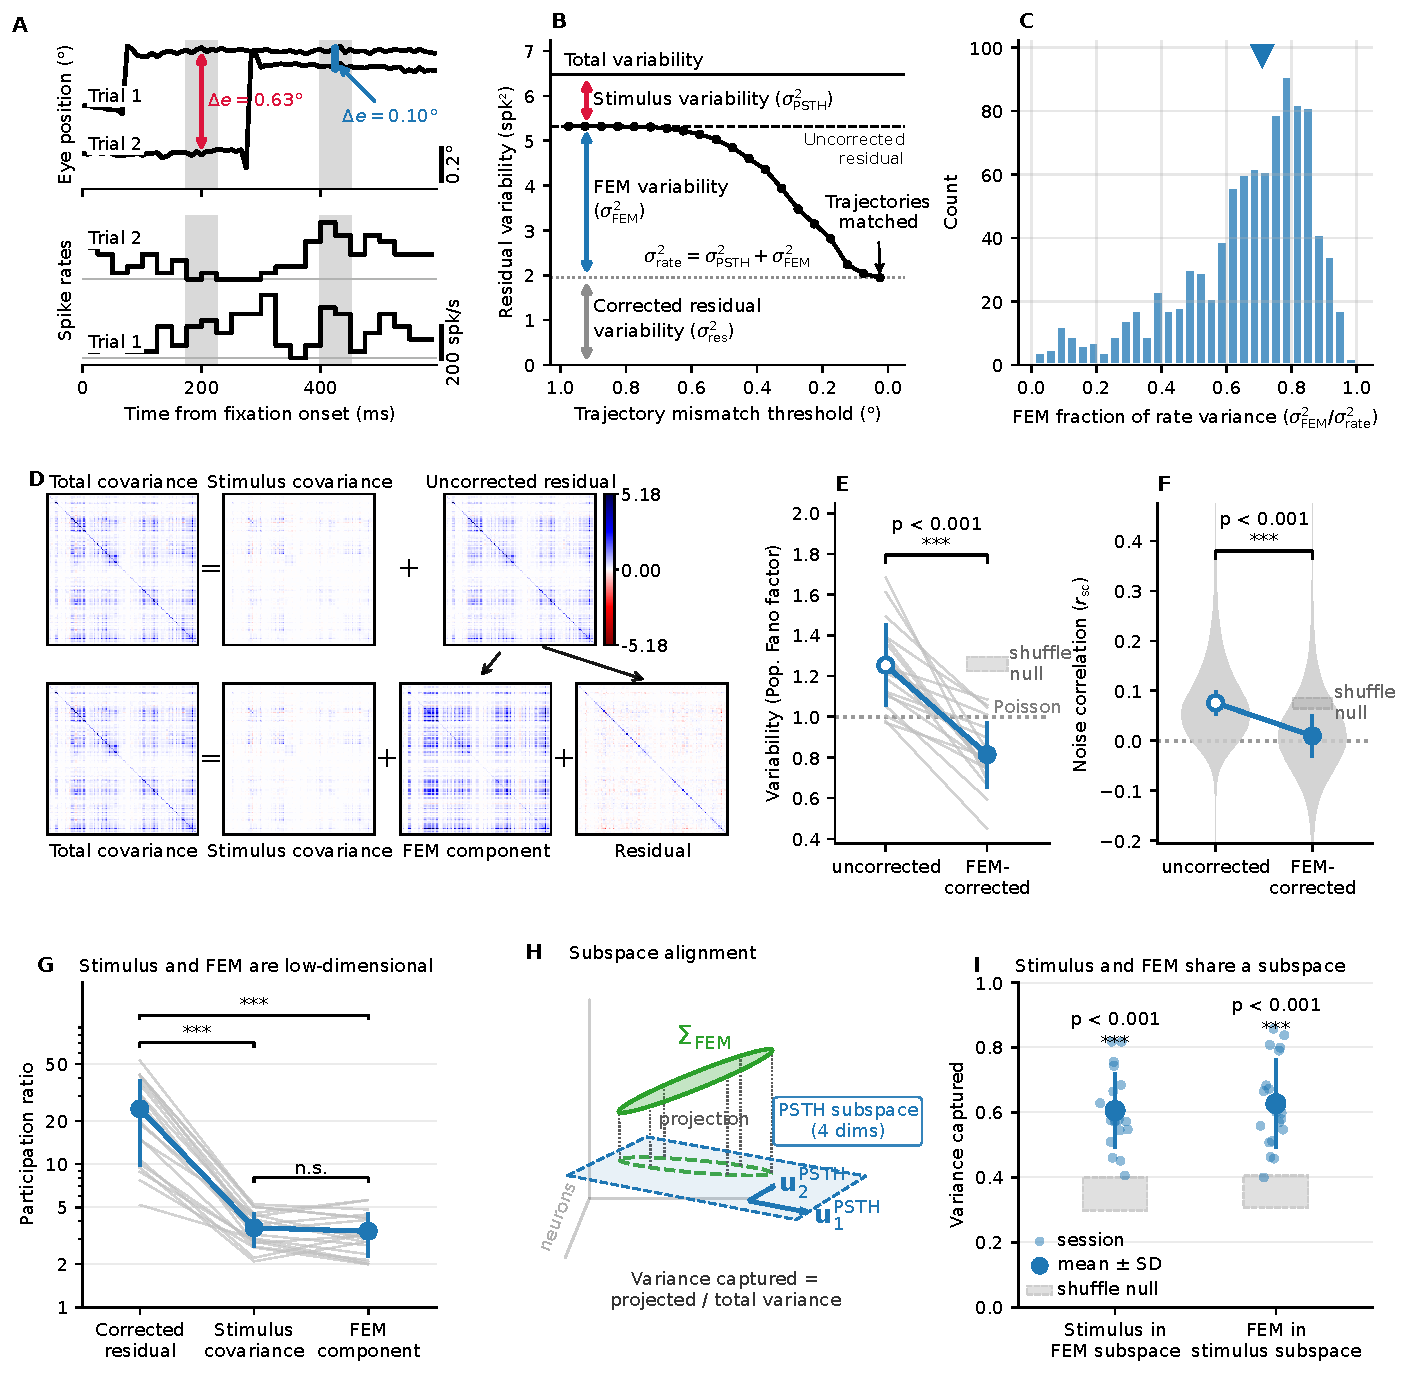
\includegraphics[width=\linewidth,height=0.78\textheight,keepaspectratio]{figures/figure2.pdf}
  \caption{
  \textbf{Fixational eye movements dominate single-neuron and shared variability, and contribute a compact population covariance component aligned with the stimulus-driven subspace.}
  }
  \label{fig:covariance}
\end{figure}

\clearpage

\begin{figure}[p]
  \ContinuedFloat
  \captionsetup{font=footnotesize,singlelinecheck=false}
  \caption{
  All panels use a 25\,ms counting window. Significance markers ($\ast$) denote comparison against the eye-trajectory shuffle null (E, F, I) or paired tests across components (G); numeric values are reported in the main text.
  \textbf{(A)} Dual-binning intuition for an example unit. At a fixed timepoint in the frozen stimulus sequence, trials are compared by the similarity of their eye trajectory. Top: eye-position traces for two trials whose gaze is closely matched at one timepoint (blue, $\Delta e = 0.10^\circ$) and divergent at another (red, $\Delta e = 0.63^\circ$). Bottom: the corresponding per-bin spike rates. Similar gaze yields similar responses, while divergent eye position yields divergent responses despite identical stimulus input.
  \textbf{(B)} Eye-attributable variability for the same unit, recovered by tightening the matching threshold. As trial pairs are required to have increasingly similar trajectories ($\Delta e < x$), the variability left unaccounted-for falls from the level attained when eye position is ignored toward an internal-noise floor. The gap (blue) is the rate variance attributable to fixational eye movements, and the fraction obscured by ignoring eye position defines $f_{\text{FEM}}$ (inset).
  \textbf{(C)} Distribution across neurons of the FEM fraction of single-neuron rate variance ($f_{\text{FEM}}$); triangles mark the per-subject medians. The distribution is biased toward one, indicating that most trial-to-trial rate variance is attributable to fixational eye movements.
  \textbf{(D)} Covariance decomposition for an example monkey~A session. Top: the conventional split, total covariance $= \Cpsth + $ classical residual, attributes all covariance not captured by the PSTH to a single internal component. Bottom: that classical residual is further partitioned into an eye-movement--dependent component $\Cfem$ and a corrected residual $\Sigma_{\text{int}}$. Off-diagonal structure in the classical residual migrates almost entirely into $\Cfem$, leaving the corrected residual near-diagonal.
  \textbf{(E)} Population Fano factor, uncorrected vs.\ FEM-corrected. Thin grey lines are individual sessions; the marker is the across-session mean $\pm$ SD. The Poisson reference (Fano $=1$) is dotted and the grey band is the shuffle null.
  \textbf{(F)} Per-pair noise correlation, uncorrected vs.\ FEM-corrected. Grey violins show the pooled per-pair distribution; the marker is the across-dataset mean $\pm$ SD and the grey band the shuffle null.
  \textbf{(G)} Participation ratio of the three covariance components --- corrected residual, stimulus-locked ($\Cpsth$), and eye-movement--dependent ($\Cfem$). One faint line per session joins its three values; the marker is the across-session mean $\pm$ SD (log scale). The stimulus and FEM components are comparably low-dimensional and far more compact than the residual.
  \textbf{(H)} Schematic of the subspace-alignment test. The low-rank FEM covariance (green disk) is projected orthogonally onto the leading eigenvectors of $\Cpsth$ (the stimulus subspace, blue plane); the fraction of variance retained, $f_{\mathrm{FEM}\to\mathrm{PSTH}} = \mathrm{tr}(U^\top\Sigma_{\text{FEM}}U)/\mathrm{tr}(\Sigma_{\text{FEM}})$, measures how much of one component lies within the other's subspace. This is one of the two directions shown in (I), and is distinct from $f_{\text{FEM}}$ in (B, C).
  \textbf{(I)} Variance captured in each direction --- stimulus-locked variance lying in the FEM subspace, and FEM variance lying in the stimulus subspace --- with one point per session and the across-session mean $\pm$ SD. The grey dashed band is the shuffle null of the mean (eye traces permuted across trials). Both directions sit well above the null, indicating that FEM-driven modulation is largely confined to the dimensions used to encode the stimulus.
  }
\end{figure}

%\begin{figure}[p]
%  \ContinuedFloat
  %\captionsetup{font=footnotesize,singlelinecheck=false}
  %\caption{
  %\textbf{(A)} Example plot of dual binning analysis, see \cite{mcfarland2016variability}, for a single unit. Eye-trajectories sampled and compared across trials for the same time point (and same stimuli) within the frozen image sequence. 
%  \textbf{(B)} Distribution of $1-\alpha$ across neurons, stacked by subject at the 8\,ms counting window. Monkey A: $n=1010$ neurons, median $0.786$ [IQR $0.670$, $0.861$]. Monkey L: $n=257$, median $0.684$ [IQR $0.541$, $0.792$]. Both distributions are skewed toward 1, indicating that most trial-to-trial rate variance is attributable to fixational eye movements.
%  \textbf{(C)} Population Fano factor vs.\ counting window, by subject (Monkey A: blue; Monkey L: green). Dashed lines/open markers show raw responses; solid lines/filled markers show FEM-corrected responses. Error bars are session-clustered bootstrap 95\% CIs; stars below each window give the per-subject corrected-vs.-uncorrected significance. Across windows and subjects, FEM correction reduces the population Fano factor toward or below the Poisson reference (gray dotted line), with larger reductions at longer counting windows.
%  \textbf{(D)} Compact covariance decomposition for an example Monkey A session at the 8\,ms counting window. Top: the conventional decomposition $\Sigma_{\text{total}} = \Sigma_{\text{PSTH}} + \Sigma_{\text{int}}^{\text{uncorr}}$ attributes all covariance not captured by the PSTH to an uncorrected internal component. Bottom: that uncorrected component is split into an eye-movement-dependent covariance $\Sigma_{\text{FEM}}$ and a residual corrected covariance $\Sigma_{\text{int}}^{\text{corr}}$. The off-diagonal structure in $\Sigma_{\text{int}}^{\text{uncorr}}$ migrates largely into $\Sigma_{\text{FEM}}$, leaving the residual covariance much closer to diagonal.
%  \textbf{(E)} Mean Fisher-$z$ noise correlation vs.\ counting window, per subject. Dashed lines/open markers show uncorrected responses; solid lines/filled markers show FEM-corrected responses. Error bars are session-clustered bootstrap 95\% CIs, with subjects dodged in $x$ for clarity. Uncorrected shared variability grows with counting window, whereas FEM-corrected correlations remain near zero at short windows and only begin to emerge at the longest window.
%  \textbf{(F)} Cumulative fraction of own variance carried by the leading eigenvalues of $\Sigma_{\text{PSTH}}$ (solid) and $\Sigma_{\text{FEM}}$ (dashed), with each session normalized to its own total variance. Thin traces are sessions; bold lines are per-subject medians. FEM spectra saturate within roughly three dimensions in both subjects, while PSTH spectra are more distributed, especially in Monkey A.
%  \textbf{(G)} Participation ratio of $\Sigma_{\text{FEM}}$ vs.\ $\Sigma_{\text{PSTH}}$, one point per session. The legend gives an exact one-sided sign test for PSTH PR $>$ FEM PR per subject. Monkey A: all 11/11 sessions fall above the diagonal, $p=5\times10^{-4}$; PR$_{\text{FEM}}$ median $2.59$ [IQR $2.38$, $3.36$] vs.\ PR$_{\text{PSTH}}$ $4.93$ [$4.10$, $5.41$]. Monkey L: 9/13 sessions fall above the diagonal, n.s.; PR$_{\text{FEM}}$ $3.14$ [$1.98$, $3.34$] vs.\ PR$_{\text{PSTH}}$ $2.86$ [$2.39$, $3.70$]. FEM variance therefore occupies roughly two to three population modes, consistent with the translational degrees of freedom of gaze.
%  \textbf{(H)} Subspace alignment between $\Sigma_{\text{PSTH}}$ and $\Sigma_{\text{FEM}}$. $X$ is the fraction of PSTH variance lying in the leading FEM subspace; $Y$ is the fraction of FEM variance lying in the leading PSTH subspace. Per-subject shuffle clouds (eye traces permuted across trials, same PSTH subspace) and their means ($\times$) sit near chance levels; observed sessions sit well above the shuffle cloud, with red outlines marking sessions jointly significant at $p<0.01$ for both $X$ and $Y$. Observed means: Monkey A $X=0.61$, $Y=0.64$ (null $0.31$, $0.25$); Monkey L $X=0.77$, $Y=0.75$ (null $0.43$, $0.48$). FEM-driven modulations are largely confined to the dimensions used to encode the stimulus. For a decoder blind to eye position this is the geometry of information-limiting correlations \cite{moreno2014information}: modulation confusable with stimulus-driven change that cannot be averaged away. For a decoder that conditions on retinal position, the same compact component is recoverable reafference rather than irreducible noise. These are two readings of one covariance in pose-blind versus pose-aware coordinates.
%  }
%\end{figure}

\clearpage

% \begin{figure}[h!]
%   \centering
%   
\includegraphics[width=\linewidth]{figures/fig2_composite.pdf}
%   \caption{
%   \textbf{Conditioning on eye position reveals a dominant contribution of fixational eye movements to single-neuron variability.}
%   \textbf{(A)} Top: horizontal eye position during two representative trials of the same frozen-stimulus sequence. Middle: the absolute difference between the two traces, $|\Delta e(t)|$. Bottom: per-bin firing rate of an example unit on the same two trials. Two windows are highlighted (gray boxes): an early window where the two eye traces diverge (large $\Delta e$) and a later window where they nearly align (small $\Delta e$). Spike-rate traces decouple inside the large-$\Delta e$ window and visibly track each other inside the small-$\Delta e$ window.
%   \textbf{(B)} For every pair of distinct trials $(i,j)$ sharing a stimulus time $t$, we compute the RMS eye-trajectory distance over a short history window and bin pairs by that distance (top: distribution of pair distances pooled across $(i,j,t)$ for this session, with the same two highlighted bins as in A). Within each bin we compute the across-pair second moment of the spike counts; subtracting the squared global mean yields the conditional rate covariance $C_{\text{eye}}(\Delta e)$ (bottom). The conditional variance grows monotonically with $\Delta e$ and asymptotes near $\mathrm{Var}(\text{PSTH})$ at large $\Delta e$ (dashed line), recovering the stimulus-locked variance given low differences in eye position. 
%   } % Optional marker
% \end{figure}

% \clearpage % Forces the next content to a new page

% \begin{figure}[t]
%     \ContinuedFloat
%     \caption{
%   \textbf{(C)} Distribution of $1-\alpha$ across neurons, stacked by subject (8\,ms counting window). Monkey A: $n=1010$ neurons, median $0.786$ [IQR $0.670$, $0.861$]. Monkey L: $n=257$, median $0.684$ [IQR $0.541$, $0.792$]. Both distributions are strongly skewed toward 1, indicating that the majority of trial-to-trial rate variance is attributable to fixational eye movements.
%   \textbf{(D)} Mean--variance relationship across neurons for Monkey A (25\,ms counting window, spk/s units; one point per neuron). Slope-through-origin fits give the population Fano factor. The uncorrected fit (dashed) is $1.435$ [95\% CI $1.360$, $1.495$]; the FEM-corrected fit (solid) is $0.702$ [$0.592$, $0.801$], well below the Poisson reference (slope 1, dotted). Bracket and stars: session-clustered bootstrap test of corrected vs.\ uncorrected slope ($\Delta = 0.733$ [$0.607$, $0.862$], $p = 5\times 10^{-4}$).
%   \textbf{(E)} Population Fano factor vs.\ counting window, by subject (Monkey A: blue; Monkey L: green). Dashed lines / open markers $=$ raw; solid lines / filled markers $=$ FEM-corrected; error bars are session-clustered bootstrap 95\% CIs; stars below each window give the per-subject corrected-vs.-uncorrected significance. Across all four windows and both monkeys, FEM correction collapses the population Fano factor below Poisson (gray dotted), and the reduction grows with counting window---consistent with eye-movement modulation accumulating over time.
%   }
%   \label{fig:covariance}
% \end{figure}


%\subsection{Covariance decomposition reveals that fixational eye movements dominate shared rate variability}


% Some reference to Figure 2A (explainer: Declan?)
%Across neurons, FEMs accounted for the majority of trial-to-trial \emph{rate} variability. We quantified this contribution using $1-\alpha$, the fraction of rate variance explained by eye movements (Methods). At a 10\,ms counting window, $1-\alpha$ was strongly skewed toward high values (median [IQR] = 0.802 [0.717, 0.868]; mean = 0.771, bootstrap 95\% CI [0.757, 0.784]; Fig.~\ref{fig:covariance}c), and exceeded a shuffle-based null that preserved stimulus timing and marginal eye statistics but destroyed trial-specific coupling (null mean 95\% CI [0.324, 0.475]; empirical $p=0.0099$). Together, these results indicate that most rate variability during fixation is predictable from measured eye movements.

%This FEM-driven structure strongly impacted classical variability metrics. After FEM correction, single-neuron Fano factors decreased substantially at short timescales (10\,ms: geometric mean 1.082 $\rightarrow$ 0.868; ratio 0.803, a 19.7\% reduction; Wilcoxon $p=4.57\times10^{-108}$; Fig.~\ref{fig:covariance}d), with reductions that persisted across counting windows up to 80\,ms (ratios 0.668 at 20\,ms; 0.527 at 40\,ms; 0.503 at 80\,ms). At the population level, we computed the population Fano factor as the slope of the mean--variance relationship across neurons \cite{churchland2010stimulus}. This quantity fell sharply after FEM correction (10\,ms: 1.082 $\rightarrow$ 0.771; $\Delta=-0.312$, bootstrap 95\% CI [$-0.354$, $-0.277$]; one-sided bootstrap $p=0.0002$; Fig.~\ref{fig:covariance}e), indicating that FEMs contribute substantially to individual neuron variability.


% Declan, need to seed the explainer text for the Covariance matrix semi-schematic/semi-data panel

%At 10\,ms, mean pairwise noise correlations shifted from positive to near zero or slightly negative (pooled pairs: mean $\rho$ 0.0520 $\rightarrow$ $-0.0087$; Fig.~\ref{fig:covariance}f). Across datasets, this corresponded to a significant reduction in Fisher-$z$--transformed correlations ($z_\text{uncorr}=0.0492$ [0.0401, 0.0583] vs.\ $z_\text{corr}=-0.0179$ [$-0.0261$, $-0.0111$]; $\Delta z=-0.0671$ [$-0.0763$, $-0.0570$]; Wilcoxon $p=6.1\times10^{-5}$; Fig.~\ref{fig:covariance}g). The effect exceeded shuffle-based null expectations (methods, null $\Delta z$ 95\% CI [$-0.0317$, 0.0042]; empirical $p=7.14\times10^{-4}$; Fig.~\ref{fig:covariance}h), confirming that the reduction reflects trial-specific coupling between eye state and population activity rather than generic smoothing or estimation bias.

% OK, here's where the "old text from which we might want to salvage some material and incorporate into the short-and-sweet main results paragraph ends

%*** returning to text that will mostly survive, but which does need substantial updates to align with updated figure/metrics

%FEM-induced fluctuations were also strongly structured. Across sessions, $\Cfem$ was consistently low-rank (participation ratio: mean $2.085\pm0.076$, median 1.985 [1.914, 2.277]; Fig. 2G) and aligned with stimulus-locked population structure. Subspace overlap between $\Cpsth$ and $\Cfem$ was high for the leading dimension (overlap $k=1$: mean $0.770\pm0.044$) and remained substantial for higher-dimensional subspaces (overlap $k=5$: mean $0.617\pm0.022$; Fig.~\ref{fig:covariance}j). 

%*** Need some text here for Panel H

%Directional variance capture further showed that the stimulus subspace captured a large fraction of FEM variance ($Y$: FEM variance captured by PSTH subspace; mean $0.753\pm0.014$), exceeding the corresponding null distribution (null $Y$ 95\% CI [0.169, 0.616]), whereas the FEM subspace captured a smaller (but still substantial) fraction of stimulus-locked variance ($X$: PSTH variance captured by FEM subspace; mean $0.675\pm0.029$; Fig. 2I). This asymmetry supports the interpretation that, in this stimulus regime, FEMs drive a low-dimensional modulation of existing stimulus-driven population patterns \cite{liska2024running} rather than introducing orthogonal shared modes of variability, consistent with an information-limiting correlation geometry \cite{moreno2014information}.

% \begin{figure}[h!]
%   \centering
%       
\includegraphics[width=\linewidth]{figures/fig3_composite.pdf}
%   \caption{
%     \textbf{Fixational eye movements account for nearly all positive noise correlations and contribute low-rank shared variability aligned with the stimulus-driven subspace.}
%     \textbf{(A)} Covariance decomposition for an example session (Monkey A, 8\,ms counting window). Top: the conventional decomposition $\Sigma_{\text{total}} = \Sigma_{\text{PSTH}} + \Sigma_{\text{int}}$ attributes everything not captured by the PSTH to an ``internal'' covariance. Bottom: the full law-of-total-covariance decomposition $\Sigma_{\text{total}} = \Sigma_{\text{PSTH}} + \Sigma_{\text{FEM}} + \Sigma_{\text{int}}$ further splits the uncorrected $\Sigma_{\text{int}}$ (arrows) into an eye-movement--dependent rate covariance $\Sigma_{\text{FEM}}$ and a residual $\Sigma_{\text{int}}$. The uncorrected $\Sigma_{\text{int}}$ inherits the strong off-diagonal structure of $\Sigma_{\text{PSTH}}$; that structure migrates almost entirely into $\Sigma_{\text{FEM}}$ after correction, leaving the residual $\Sigma_{\text{int}}$ nearly diagonal.
%     \textbf{(B)} Pairwise noise correlations $\rho$ at the 8\,ms window, FEM-corrected vs.\ uncorrected, one dot per neuron pair; filled marker gives the per-monkey mean. Monkey A ($n=55{,}718$ pairs): mean $\rho$ shifts from $0.040$ uncorrected to $0.003$ FEM-corrected. Monkey L ($n=3{,}867$): $0.040 \rightarrow 0.007$. The broad positive uncorrected cloud collapses onto the horizontal axis after FEM correction.
  
%   } % Optional marker
% \end{figure}

% \clearpage % Forces the next content to a new page

% \begin{figure}[t]
%     \ContinuedFloat
%     \caption{
%         \textbf{(C)} Mean Fisher-$z$ noise correlation vs.\ counting window, per subject (Monkey A blue, Monkey L green; dashed/open $=$ uncorrected, solid/filled $=$ FEM-corrected; error bars are session-clustered bootstrap 95\% CIs; subjects dodged in $x$ for clarity). Uncorrected $z$ grows roughly threefold from 8 to 50\,ms, consistent with eye-movement modulations integrating over time; FEM-corrected $z$ remains near zero at short windows and only emerges at 50\,ms. 
%         \textbf{(D)} Effect size $\Delta z = z_{\text{corr}}-z_{\text{uncorr}}$ vs.\ window, plotted against the per-subject shuffle null 95\% band (shaded; eye traces permuted across trials). Stars below each window give per-subject empirical $p$-values relative to that null (***\,$p<10^{-3}$, **\,$p<10^{-2}$, *\,$p<0.05$). Observed $\Delta z$ is negative and falls well outside the null at every short window (8\,ms: Monkey A $\Delta z = -0.041$, $p = 9\times 10^{-4}$; Monkey L $-0.037$, $p = 3\times 10^{-3}$), confirming the reduction reflects trial-specific eye/spike coupling rather than smoothing or estimator bias.
%         \textbf{(E)} Cumulative fraction of own variance carried by the leading eigenvalues of $\Sigma_{\text{PSTH}}$ (solid) and $\Sigma_{\text{FEM}}$ (dashed); each session normalized to its own total. Thin traces are sessions, bold lines are per-subject medians. FEM spectra saturate within $\sim$3 dimensions in both subjects; PSTH spectra are systematically higher-dimensional, especially in Monkey A.
%         \textbf{(F)} Participation ratio of $\Sigma_{\text{FEM}}$ vs.\ $\Sigma_{\text{PSTH}}$, one point per session. Legend gives an exact one-sided sign test for PSTH PR $>$ FEM PR per subject. Monkey A: all 11/11 sessions above the diagonal, $p=5\times 10^{-4}$; PR$_\text{FEM}$ median $2.59$ [IQR $2.38$, $3.36$] vs.\ PR$_\text{PSTH}$ $4.93$ [$4.10$, $5.41$]. Monkey L: 9/13 sessions above the  diagonal, n.s.; PR$_\text{FEM}$ $3.14$ [$1.98$, $3.34$] vs.\ PR$_\text{PSTH}$ $2.86$ [$2.39$, $3.70$]. FEM variance lives in roughly two to three population modes, consistent with the translational degrees of freedom of binocular gaze.
%         \textbf{(G)} Subspace alignment between $\Sigma_{\text{PSTH}}$ and $\Sigma_{\text{FEM}}$: $X$ is the fraction of PSTH variance lying in the leading FEM subspace, $Y$ the fraction of FEM variance lying in the leading PSTH subspace. Per-subject shuffle clouds (eye traces permuted across trials, same PSTH subspace) and their means ($\times$) sit near the diagonal at chance levels; observed sessions (filled markers) sit well above the cloud, red outlines marking sessions jointly significant at $p<0.01$ for both $X$ and $Y$ (Monkey A 11/11; Monkey L 11/13). Observed means: Monkey A $X=0.61$, $Y=0.64$ (null $0.31$, $0.25$); Monkey L $X=0.77$, $Y=0.75$ (null $0.43$, $0.48$). FEM-driven modulations are largely confined to the dimensions used to encode the stimulus, supporting an information-limiting correlation geometry rather than orthogonal shared noise.
%   }
%   \label{fig:covariance}
% \end{figure}


\subsection{Active visual sensing is implemented via an eye-brain-environment feedback loop}

The prior analyses show that FEM-driven modulation occupies the same low-dimensional subspace as the stimulus response, but they do not identify the source of that modulation. One possibility is reafference: fixational eye movements physically displace the image on the retina, and V1 follows the resulting change in retinal input. A second possibility is extraretinal modulation: an efference copy or proprioceptive estimate of eye position could modulate V1 independently of the image on the retina. These accounts could produce similar population geometry but assign the variability to fundamentally different sources.

To distinguish between these two possibilities, we fit a single image-computable recurrent deep neural network model to the recorded V1 population. The model was trained to predict responses to gratings, Gabors, and natural images during free viewing \cite{yates2023detailed} and evaluated on the rapid serial image presentation condition analyzed previously (Fig.~3a). This model predicts neural responses from two inputs: retinal input and behavioral input. The retinal input is a gaze-contingent reconstruction of the stimulus over time, so fixational eye movements implicitly enter the model as motion of the retinal image. The behavioral input contains eye position and velocity and explicitly enters the model as a distinct component before a recurrent modulatory stage (Fig.~3b). This behavioral pathway is the only route by which eye state can influence the response without moving the retinal image. This statistical account of the neural responses conditioned on these two inputs supports model comparisons where we selectively ablate either the effect of eye movements from the retinal or behavior (extra retinal) pathways. By setting the behavior inputs to zero, we can test whether the model needs a separate extraretinal eye-state signal after the retinal image motion has already been specified. In a complementary manipulation, we froze the retinal input at each trials median gaze position while leaving the behavioral input intact. This stabilized condition removes image motion caused by fixational eye movements, and thus the reafferent signal, while preserving extraretinal eye-position and velocity signals.

The full model reproduced the trial-averaged responses across the recorded population equivalently to other state-of-the-art models of visual cortex \cite{wang2025foundation} (median $\mathrm{CC_{norm}} = 0.664$, IQR $[0.517, 0.788]$; $n = 984$ cells across both monkeys; Fig.~3c). Removing the extraretinal pathway produced a consistent but small decrease in trial-averaged prediction (median $0.643$; paired $\Delta \mathrm{CC_{norm}} = -0.014$, a $2\%$ reduction; $p = 1.6\times10^{-44}$). Stabilizing the retinal input had a larger effect (median $0.504$; paired $\Delta \mathrm{CC_{norm}} = -0.143$, a $21\%$ reduction; $p = 1.2\times10^{-136}$), although much of the trial-averaged response remained predictable. However, the effects measured in previous sections are not changes in the mean response. FEMs organize the variability around that mean, which the trial average discards.

We therefore scored each predictor on single trials, as the fraction of the explainable rate variance measured in Figure~2 that it captured (Methods). This fraction is zero for a predictor that captures no rate modulation and one for an ideal predictor of the gaze-conditional rate, which places the leave-one-out trial average and the three twin conditions on a common scale. This comparison is deliberately stringent. The trial average is often treated as a practical ceiling for image-computable models, because it contains the repeatable stimulus-locked response and averages away trial-to-trial fluctuations. However, the trial average captured a median of just $0.157$ of the rate variance, while the full twin captured $0.269$, a $67\%$ gain (paired $\Delta = +0.106$; $n = 972$ cells from 19 sessions; session-level Wilcoxon $p = 0.032$; Fig.~3d). This demonstrates that the full model captured structure in individual trials that was absent from the trial average. 

We then tested whether this gain in trial-by-trial variance explained was driven primarily by retinal or behavioral input. The retinal-only twin, with eye position and velocity zeroed, retained nearly all of the full model advantage (median $0.246$; paired $\Delta = -0.014$, $p = 0.35$) and remaining above the trial-average reference ($\Delta = +0.085$, $p = 0.011$). By contrast, stabilizing the retinal input cut the explained fraction to $0.042$, a loss of $72\%$ ($\Delta = -0.193$, $p = 3.8\times10^{-6}$), and dropped the twin below the trial average ($\Delta = -0.114$, $p = 1.6\times10^{-4}$). Single-trial prediction therefore depended on retinal image motion, and the separate extraretinal input contributed little.

We then asked whether the twin reproduced the FEM modulation measured directly from the neurons, applying the Figure~2 decomposition to each condition's predicted rates (Methods). The full and retinal-only twins matched the empirical distribution, with medians of $0.618$ and $0.631$ against an empirical $0.652$ and paired offsets of only $0.026$ and $0.024$, both equivalent within a $\pm0.1$ margin (paired TOST, both $p < 10^{-29}$; Fig.~3e). Stabilizing the retinal input shifted the model median to $0.196$, well outside that margin (median paired difference $0.402$; paired signed-rank $p = 3.8\times10^{-93}$). Retinal image motion was therefore sufficient to reproduce the magnitude of FEM-driven rate modulation, and removing that motion abolished it.

These results identify the FEM-dominated foveal code as a reafferent signature of active sensing. Fixational eye movements shape V1 activity by continuously moving the image across the retina. The moving retinal input is sufficient to retain the model's single-trial advantage when the extraretinal pathway is removed and necessary for prediction to exceed the trial-average baseline when extraretinal behavior remains available.

%Although the neural population activity subspaces occupied by the visual stimulus and by FEMs were low dimensional and shared, that observation does not directly tell us whether FEM-related variability reflects low-dimensional feedback signals (i.e., efference copies of the FEMs), or a direct consequence on visual stimulation (i.e., ``reafference'', by changing the retinal input). To more fully understand the relation between FEMs and neural variability, we fit a shared image-computable deep neural network (DNN) to all neurons during free-viewing natural scenes and noise stimuli \cite{yates2023detailed} to use as a digital twin for the population (Fig 3a). The DNN captured the receptive field properties of the cells (Fig 3b) and PSTH to the withheld fixation condition (Fig 3c). The average noise-corrected correlation of 0.70 [XX,XX] on capturing the mean response to the fixation condition (Fig 3d).  To examine the role of fixational eye movements, we compared the trial-by-trial variance explained by the model to the variance explained by the PSTH. We found that the image-compatible model retinal input jittered with the real eye movements consistently explained more trial-by-trial variance than the PSTH (Fig 3e). Further, the fixational eye movement variability lived in a shared subspace with the stimulus tuning of the DNN (Fig 3f). This suggests that a substantial portion of the variability due to eye movements is in the retinal input itself.


\begin{figure}[t]
  \centering
  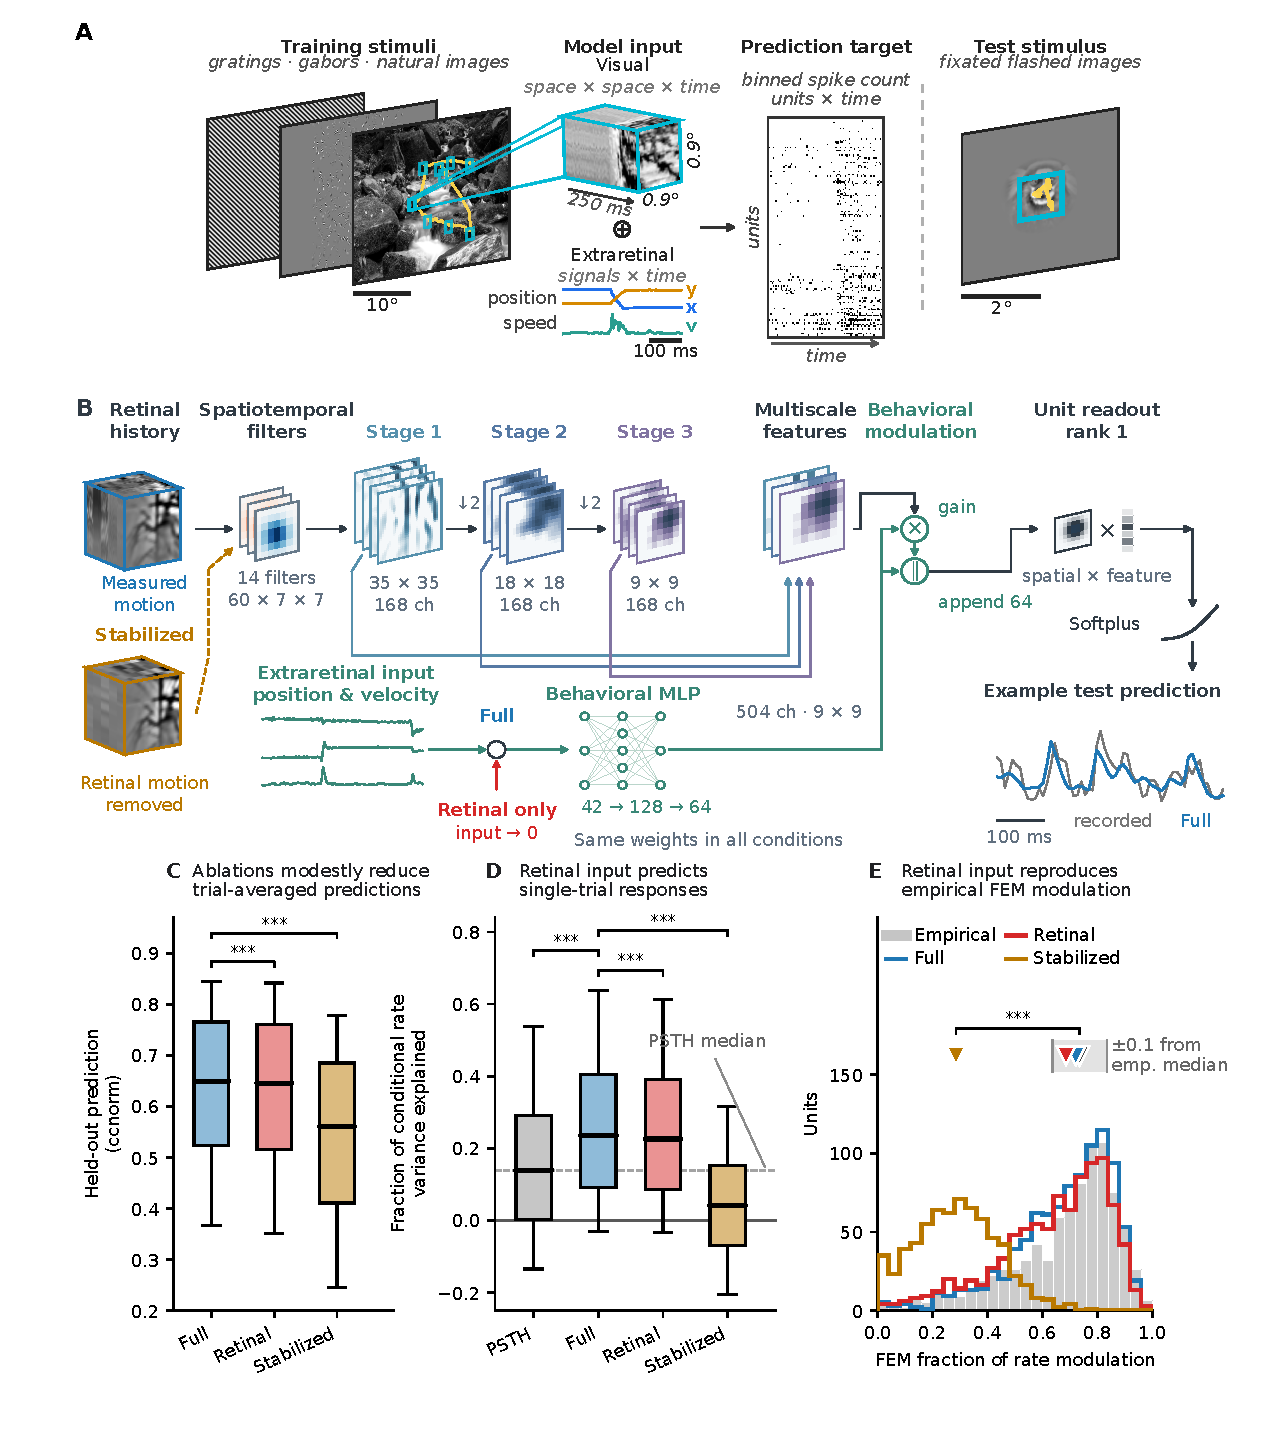
\includegraphics[width=\linewidth]{figures/figure3.pdf}
  \caption{
  \textbf{An image-computable digital twin reproduces eye-movement driven variability through feedforward computation on retinal input}
    } % Optional marker
\end{figure}
\begin{figure}[t]
  \ContinuedFloat
  \captionsetup{font=footnotesize,singlelinecheck=false}
  \caption{
    \textbf{(A)} Stimuli and retinal input. The digital twin is trained on
    grating, Gabor, and natural image stimuli during free viewing, and evaluated on the held-out flashed image dataset. Its input is the gaze-contingent retinal stimulus, a space $\times$ space $\times$ time reconstruction of the stimulus history accounting for measured eye position, as well as eye position and velocity measurements.
    \textbf{(B)} Model architecture. A shared convolutional--recurrent core (ResNet $\rightarrow$ ConvGRU) maps the retinal stimulus sequence to each unit's firing rate through a per-unit Gaussian readout. A separate extraretinal input supplies eye position and velocity. The retinal-only condition zeroes this extraretinal input while retaining the gaze-contingent retinal sequence. The extraretinal-only (stabilized) condition freezes the retinal input for all trials at one session-global gaze centroid while retaining the behavioral input, thereby removing reafferent image motion.
    \textbf{(C)} Held-out, trial-averaged prediction (noise-normalized correlation, $\mathrm{CC_{norm}}$) for the full, retinal-only, and extraretinal-only twins ($n=984$ cells across 19 sessions). Removing the extraretinal input lowers prediction slightly. Stabilizing the retinal input causes a larger reduction.
    \textbf{(D)} Single-trial prediction as a fraction of the explainable rate variance measured in Figure~2. The leave-one-out trial average and all three twin conditions are shown ($n=972$ cells across 19 sessions). The full twin exceeds the trial average. The retinal-only twin retains the full prediction, whereas stabilizing the retinal input reduces the explained fraction. The dashed line marks the trial-average median and the solid line marks zero captured variance. Values above one were retained rather than clipped because the denominator is an estimate, not a hard upper bound.
    \textbf{(E)} Distribution of the FEM modulation fraction, $f_{\mathrm{FEM}}$, for the recorded neurons and each twin condition. Downward triangles mark distribution medians. The empirical median was $0.652$, compared with $0.618$ for the full twin, $0.631$ for the retinal-only twin, and $0.196$ for the stabilized twin. The shaded band shows the empirical median $\pm0.1$. Paired two-one-sided tests with this equivalence margin supported equivalence for the full and retinal-only twins (both $p<10^{-29}$), but not for the stabilized twin ($p=1.0$). The empirical and stabilized estimates differed by a median of $0.402$ (paired Wilcoxon $p=3.8\times10^{-93}$). In C and D, boxes span the interquartile range, median lines mark the medians, and whiskers span the 10th--90th percentiles across cells.
  }
  \label{fig:twin}
\end{figure}


\clearpage

%\subsection{Fixational eye movements modulate temporal signals to sharpen spatial information}
\subsection{Fixational eye movements sharpen spatial population codes}

Sensor motion is ordinarily associated with a loss of spatial precision. A conventional camera exposure averages together together shifted images generated by motion, blurring edges and reducing spatial contrast. It has been debated whether the visual system behaves similarly \cite{gur2024seeing, rucci2025visual}. Leveraging our model of V1, we therefore asked whether the jittered retinal input generated by fixational eye movements blur cortical activity or, counterintuitively, may sharpen it. The results were decisive: compared with counterfactually stabilized input, natural retinal motion produced activation maps with stronger and more spatially concentrated responses (Fig. 4A). Thus, the same movements that introduce temporal variation into the retinal input can sharpen its spatial representation in V1.

To quantify this effect, we used the digital twin to construct model-derived populations of co-tuned neurons tiled across visual space. For each fitted unit, we replicated its spatial readout at every position within the modeled visual field, producing an activation map whose values represent the responses of neurons with the same tuning but different receptive-field locations. We quantified the information contained in each instantaneous population map by computing single-spike information across space (SSI; see Methods), defined as the divergence of the activation map from a uniform distribution. SSI is insensitive to overall response magnitude and instead captures how activity is selectively distributed across the simulated population. A diffuse map, in which activity is distributed broadly across many locations, has low SSI. Conversely, a non-uniform map with localized spatial structure has high SSI, such that the identity of an active neuron carries more information for a downstream decoder. We therefore refer to increases in SSI as sharpening of the spatial population code.

\begin{figure}[p]
  \centering
  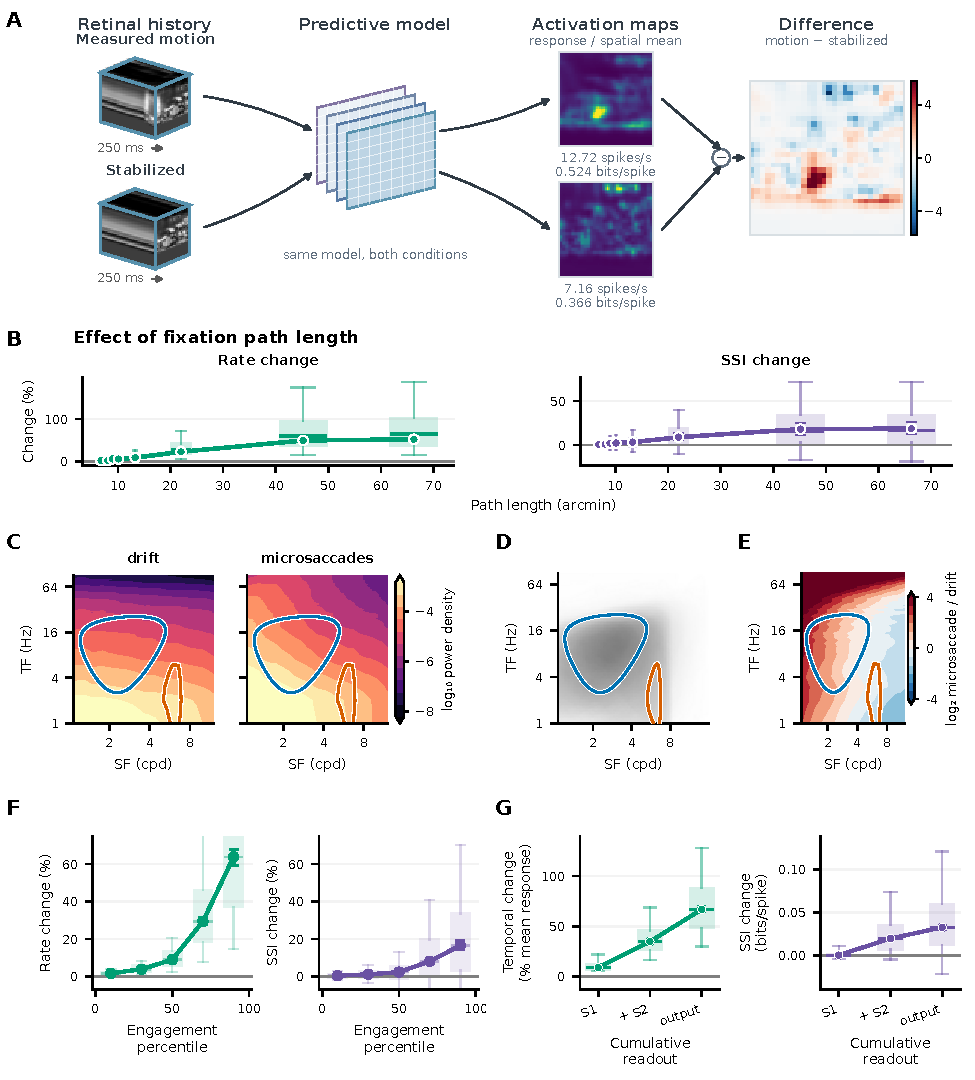
\includegraphics[width=\linewidth]{figures/figure4.pdf}
  \caption{
  \textbf{Fixational eye movements sharpen spatial coding according to neuronal tuning and local image structure.}
    } % Optional marker
\end{figure}

\begin{figure}[p]
  \ContinuedFloat
  \captionsetup{font=footnotesize,singlelinecheck=false}
  \caption{
    \textbf{(A)} Model-based single-spike information (SSI) analysis. For each fitted unit, the learned readout was translated across the spatial dimensions of the model feature grid, yielding a response at every location rather than only at the fitted receptive-field. The resulting activation map represents a spatially tiled population of neurons with the same feature tuning but different receptive field locations. Together, maps from 100 representative modeled units selected to minimize redundancy approximate a broader V1 population spanning feature tuning and visual-field position. SSI quantifies the spatial concentration of each activation map as its divergence from a uniform response distribution, in bits per spike; larger values indicate a sharper spatial population code. Each scored output used a 32-frame (267-ms) input history, and population analyses aggregated 40 successive outputs whose centers spanned 0.325~s. Example activation maps and SSI values are shown for FEM-jittered (top) and counterfactually stabilized (bottom) movies. In the example, the FEM-jittered movie produces a more concentrated activation map and higher SSI than its counterfactually stabilized counterpart.
    \textbf{(B)} SSI change from the image- and unit-matched stabilized baseline as a function of total FEM path length for low-spatial-frequency units (low-SF; $<0.5$ cycles/degree; $n=71$ units, $7{,}100$ unit--image pairs) and high-spatial-frequency units (high-SF; $\geq0.5$ cycles/degree; $n=29$ units, $2{,}900$ pairs). Open markers denote drift-only trajectories, filled markers denote trajectories containing microsaccades, and the point at zero denotes the stabilized condition.
    \textbf{(C)} A Sobel-gradient structure tensor computed within a gaze-centered, one-degree-radius image patch defined the local contour axis and edge coherence. Examples show the four coherence bins used below. Subsequent analyses examine how modeled information depends on the relationships among three axes: unit orientation preference, local contour axis, and the major axis of the eye-position cloud.
    \textbf{(D)} Path-length dependence for unit--image pairs in which unit orientation preference was aligned with the local contour (low-SF: $n=57$ units, $977$ pairs; high-SF: $n=22$ units, $356$ pairs). Marker fill is as in (B).
    \textbf{(E)} SSI change from stabilization for intact two-dimensional drift trajectories grouped by their RMS position spread across (solid lines, circles) or along (dashed lines, squares) the local contour in the aligned high-SF population. These projections were used only to summarize and bin trajectories; the model always received the intact two-dimensional trajectory. The gray band marks the interquartile range of component RMS values in the drift-only real-trace bank (1.22--1.72~arcmin), pooled across the two projections; values $>3.8$~arcmin are omitted for visual clarity. Printed $p$-values are from two-sided image-bootstrap tests comparing the first nonzero bin with stabilization and comparing the across- and along-contour conditions at the largest matched dose.
    \textbf{(F)} Contour-relative RMS position spread for $11{,}749$ fixation windows across 30 sessions. Centered eye positions were projected onto axes ranging from parallel to orthogonal to the local contour. Dashed lines show references obtained by scrambling contour orientations within each coherence bin.
    \textbf{(G)} Marginal-curve estimate of the SSI advantage conferred by the observed contour--trajectory pairing relative to random rotations of the same eye-position cloud. For each window, the contour-relative RMS values were interpolated through the across- and along-contour curves in (E), and the two resulting SSI estimates were averaged. Thus, this quantity is not a direct model evaluation of a two-dimensional SSI surface. Positive values favor the observed pairing. Open markers denote estimates whose 95\% CIs include zero.
    \textbf{(H)} Spatial scale of contour-following behavior. At each patch radius, the plotted regression slope relates edge coherence to the alignment index $\cos(2\Delta\theta)$ among windows with coherence $>0.3$, where $\Delta\theta$ is the axis-angle difference between the eye-position cloud and the local contour. Error bars in (B), (D), and (E) are 95\% image-bootstrap CIs; those in (G) are paired-window bootstrap CIs, and those in (H) are 95\% CIs on the regression slopes.
  }
  \label{fig:ssi}
\end{figure}



FEMs increased SSI across two broad classes of spatial tuning, but the dependence on movement amplitude differed substantially between them. Across low-spatial-frequency units (N units; pref. spatial frequency $<$ XX cpd), SSI increased progressively with trajectory path length, and trajectories containing microsaccades produced larger gains than drift-only trajectories of comparable length (N units;  XXXX unit–trajectory pairs; Fig. 4B). High-spatial-frequency units (N units; pref. spatial frequency $>$ XX cpd) also benefited from retinal motion, but over a more restricted range. In this population SSI was greatest at intermediate path lengths and declined for the longest trajectories (N units; Fig. 4C). Retinal stabilization was therefore not the most informative condition for either population, but neither was greater motion universally better. The movement that benefits a neuron depends on the spatial scale to which it is tuned.

This dependence on the tuning of the neuron became more pronounced when we considered the local structure of the image. We identified image regions containing a coherent local contour and restricted the analysis to units whose orientation tuning was aligned with that contour (Fig. 4D). Low-spatial-frequency aligned units retained the population-wide pattern: longer trajectories and microsaccades produced progressively larger increases in SSI (Fig. 4E). High-spatial-frequency aligned units behaved differently. Small movements produced modest benefits, but longer paths—particularly those containing microsaccades—reduced SSI and could drive it below the stabilized baseline (Fig. 4F). The average benefit observed across all high-spatial-frequency units therefore conceals a specific cost to the neurons carrying fine information about the local contour.

This interaction follows from the geometry of retinal motion. Retinal displacement converts spatial variation into temporal modulation, and the modulation experienced by an oriented neuron depends on the component of motion across its preferred spatial structure. Motion across a contour sweeps its luminance profile through the receptive field, whereas motion along the contour produces much less change in the feature encoded by a contour-aligned unit. Accordingly, SSI in high-spatial-frequency aligned units depended strongly on the across-contour component of the trajectory: small across-contour excursions increased information, but larger excursions progressively degraded it (Fig. 4G,H). The dependence on across-contour excursion was significant (p=0.XX), whereas the effect of along-contour excursion was substantially weaker and did not reach significance (p=0.XX). Total path length is therefore not sufficient to predict the coding consequence of an eye movement. Its effect depends jointly on movement amplitude, movement direction, local image structure, and neuronal tuning.

Natural FEMs exhibited precisely this directional structure. Around coherent contours, gaze positions were distributed more broadly parallel to the local contour and more narrowly in the orthogonal direction, with the anisotropy increasing as local edge coherence increased (Fig. 4I). This arrangement permits relatively large overall movement while limiting the across-contour displacement that is most costly to high-spatial-frequency aligned units. Relative to a control that randomized the orientation of the trajectory with respect to the local image, the observed trajectories preferentially increased SSI in the aligned high-spatial-frequency population (Fig. 4J). The benefit was not uniform across all channels: it was largest for the population whose fine-scale tuning matched the local image structure. FEM statistics therefore appear to distribute motion-dependent information selectively across cortical subpopulations rather than maximizing the response of every neuron simultaneously.

%The preceding results establish that FEMs drive foveal V1 through reafference. They do not address what that reafference contributes. Because the retinal consequence of an eye movement depends jointly on the trajectory and the image, and because trajectories cannot be imposed on a behaving animal, we used the model as a surrogate population in which both are under experimental control.

%The model predicts the responses of n recorded neurons to any retinal movie. By replicating each neuron's readout spatially, we end up with a complete digital twin of V1 neurons over a patch of retinal input. We treat the resulting activation map for each fitted unit as a pseudopopulation of V1 neurons sharing tuning but differing in receptive field location, and quantify the spatial information in each map as the KL divergence between the normalized map and a uniform map — the spatial analogue of single-spike information. A flat map carries no information about where structure lies in the image; a sparse, peaked map carries a great deal [Fig 4A inset].

%Stabilized input produced the least informative maps for every unit class (Fig.~\ref{fig:ssi}B). Replacing the stabilized input with real fixational trajectories sampled from the same animals increased spatial information by \ph{X\%, IQR} for low-spatial-frequency units and \ph{X\%, IQR} for high-spatial-frequency units. The dependence on trajectory amplitude differed sharply between them. Low-spatial-frequency units gained monotonically with path length and gained most when the trajectory contained a microsaccade. High-spatial-frequency units peaked at \ph{X} arcmin of drift and lost information beyond it, so that the trajectories most informative for one population were among the least informative for the other.
 
%A single mechanism accounts for both profiles. Retinal motion converts spatial structure into temporal modulation: a unit with preferred spatial-frequency vector $\mathbf{k}$ moving at velocity $\mathbf{v}$ experiences temporal frequency $f_t = \mathbf{v}\cdot\mathbf{k}$. Units with a temporal passband are therefore driven best by the velocity that places $f_t$ inside it, and that velocity scales inversely with preferred spatial frequency \cite{rucci2015unsteady,rucci2018temporal}. We measured each model unit's temporal tuning directly by probing the twin with drifting gratings (Fig.~\ref{fig:ssi}C), finding preferred temporal frequencies of \ph{X} Hz \ph{range} and preferred spatial frequencies spanning \ph{X--X} cycles per degree. Recomputing the trajectory dependence against experienced temporal frequency rather than path length collapsed the low- and high-spatial-frequency curves onto a common function peaking at \ph{X} times each unit's preferred temporal frequency (Fig.~\ref{fig:ssi}D; variance explained by the collapsed fit \ph{X}, versus \ph{X} for the path-length parameterization). The apparent disagreement between the two populations reflects a single shared preference expressed through different spatial scales.
 
%Because $f_t$ is a projection, direction is as consequential as amplitude. We tested this on synthetic contours of controlled spatial frequency, presenting trajectories confined to lie along or across the contour axis (Fig.~\ref{fig:ssi}E). Units carrying the contour are those whose $\mathbf{k}$ lies along its normal, for which along-contour motion gives $\mathbf{v}\cdot\mathbf{k}=0$. Spatial information in these units was unchanged by along-contour motion at any amplitude ($\Delta = \ph{X}$, \ph{n.s.}), and was tuned for across-contour motion, peaking at \ph{X} arcmin and declining thereafter (Fig.~\ref{fig:ssi}F). The optimal across-contour amplitude scaled as the inverse of the contour's spatial frequency (slope \ph{X} on logarithmic axes, \ph{CI}), confirming that the tuning follows temporal frequency rather than displacement.
 
%The two directions therefore carry asymmetric cost. Motion across a contour must be held within a narrow range to serve the units encoding it, while motion along a contour is unconstrained for those units and continues to benefit units tuned to other image content. Under a fixed drift budget, the allocation maximizing population spatial information is anisotropic, with \ph{X}-fold more motion along contours than across them (Fig.~\ref{fig:ssi}G).
 
%We asked whether marmosets show this asymmetry during free viewing of natural scenes. For each fixation we estimated the dominant orientation and its coherence within the central \ph{1}$^\circ$ and measured the spread of gaze relative to that axis, referenced to a baseline in which image orientation was randomized while gaze was left intact. Drift was anisotropic in the predicted direction: position spread exceeded baseline parallel to the contour and fell below it orthogonally, with the effect growing from \ph{X} arcmin in the lowest coherence bin to \ph{X} arcmin in the highest (Fig.~\ref{fig:ssi}H,I; $p < \ph{X}$). Passing the observed and orientation-randomized trajectories back through the twin, the observed anisotropy corresponds to a \ph{X\%} increase in population spatial information (Fig.~\ref{fig:ssi}J).
 
% ---- Closing sentence: choose one once the bridge number is in hand. ----
 
% Use if the effect is large:
% Fixational drift is thus shaped to the spatial content of the image in a
% manner that preserves the information available to the foveal population.
 
% Default until the number says otherwise:
%Marmoset drift is therefore biased, if modestly, toward the trajectory statistics that preserve high-spatial-frequency information, indicating that oculomotor control near the fovea is sensitive to the same image variable that governs cortical encoding.

\section{Discussion}

%[LLM generated; requires heavy editing for prose and content]

%Fixational eye movements accounted for most explainable single-neuron rate variance and much of the shared variability in the foveal representation of V1. This activity was low-dimensional, occupied stimulus-responsive population dimensions, and was reproduced by an image-computable model through gaze-contingent retinal input. In model-derived populations, natural retinal motion also increased spatial single-spike information relative to stabilization, with benefits that depended on movement, image structure, and neuronal tuning. The common source of these effects is the retinal sequence generated during fixation. Eye movements continually transform the input, V1 responds to those transformations, and the resulting variation changes the spatial information expressed across the population.

%This coupling is especially consequential for primate vision. High-acuity vision is concentrated in the fovea, so primates repeatedly place a small retinal region over behaviorally relevant image structure. Our results show that the ensuing fixation does not suspend the sensorimotor process. Movements during nominal fixation remain large relative to the spatial sensitivity of foveal neurons and drove more rate modulation than the repeated sequence of displayed images. The retinal input to foveal V1 therefore continued to depend on the animal's behavior even when gaze appeared stable and no overt sampling movement was required by the task. Previous work showed that FEMs alter V1 responses and support fine spatial judgments \cite{mcfarland2016variability,rucci2007miniature}. The present population measurements connect these observations by demonstrating that active sampling plays an outsized role in shaping the cortical representations of visual input at the foveal, at least in the primary visual cortex.

%The source of this modulation clarifies what makes the sensing active. Motor commands may changes the eye's position, but the resulting neural input also depends on the structure of the image through which the eye moves. The returning signal is therefore generated jointly by the animal and its environment. Our model captured this interaction without requiring a separate representation of eye state. Removing the behavioral eye-position and velocity inputs preserved single-trial prediction and the empirical magnitude of FEM modulation, whereas stabilizing the retinal image removed both effects. Within the model, retinal image motion was sufficient and the explicit extraretinal pathway contributed little. This does not exclude efference copy, proprioception, or eye-related modulation elsewhere in the visual system. However, it does demonstrate that extraretinal modulation is unnecessary to explain large eye-movement related signals in foveal V1. Human psychophysics supports the same separation: retinal motion benefits fine discrimination even when decoupled from the observer's current eye trajectory \cite{ratnam2017benefits}, and retinal motion cues can support perceptual stability during drift without a precise estimate of eye position \cite{poletti2010stability}. The eye--brain loop closes through the environment because each movement acts on a particular image and returns a new retinal input to cortex.

%This external loop changes the interpretation of cortical variability. Repeated presentations of a display are conventionally treated as repeated sensory inputs, with deviations from the trial average assigned to internal neural variability. During fixation, however, the animal generates a different retinal sequence on every trial. Accounting for that sequence reduced the population Fano factor from $1.24$ to $0.80$ and the mean pairwise correlation from $0.077$ to a value indistinguishable from zero. Much of the apparent noise under these conditions was structured sensory variation omitted from the experimental description. Its alignment with stimulus-responsive dimensions follows from its physical origin: movement changes which part of the image falls on each receptive field. A decoder that ignores gaze can confuse this reafferent variation with a change in the displayed image. Subspace alignment alone does not establish the differential-correlation geometry required for an irreducible information limit \cite{kanitscheider2015origin}. It instead shows that the variables normally separated as stimulus and behavior converge in the population response. For foveal vision, specifying the screen stimulus while marginalizing over gaze leaves a central determinant of the neural input unobserved.

%The coding consequences also show why continuous active sensing cannot be reduced to added jitter. Retinal motion did not affect every channel uniformly. In model-derived populations of spatially tiled, co-tuned neurons, longer trajectories generally increased spatial information among low-spatial-frequency units. Fine-scale, contour-aligned units benefited over a narrower range and lost information when motion carried the contour too far across their preferred structure. Natural trajectories around coherent contours limited this costly across-contour displacement while allowing more motion along the contour. Eye movements therefore redistributed spatially selective activity across neural subpopulations as the trajectory evolved. This dynamic allocation is well suited to a foveal system in which different image features enter the high-acuity representation from moment to moment. It also implies that no single movement statistic is beneficial in isolation. The coding effect depends on the movement relative to the current image and the tuning of the neurons that sample it.

%These observations extend the active-sensing account of primate vision in two ways. First, active sensing remains engaged during fixation, when conventional experiments most often assume stable input. Second, the relevant feedback loop extends beyond the nervous system: motor output changes the retinal image through the structure of the external scene, and that reafferent sequence organizes cortical activity. Tests across eccentricity, visual areas, and task demands will be needed to establish how downstream populations use this structure. The central implication is already present at the first cortical stage. Foveal V1 encodes an input continuously constructed by image structure and self-generated movement. Active sensing is therefore an ongoing condition of primate foveal vision, including within every fixation.

\section{Methods}

The present study analyzed recordings from two adult male common marmosets (Callithrix jacchus), referred to as monkeys L and A. Recordings from monkey L were collected as part of the dataset described by Yates et al. \cite{yates2023detailed}. Recordings from monkey A were collected subsequently using the same experimental preparation and acquisition system, with minor modifications, as described below. The fixated flashed-image condition analyzed here was not described in the previous report. We therefore summarize the shared data-collection procedures and describe this condition separately.

All surgical and experimental procedures were approved by the Institutional Animal Care and Use Committee at the University of Rochester and conformed to US National Institutes of Health guidelines. As described previously \cite{yates2023detailed}, each animal was implanted with a titanium head post and a recording chamber positioned over V1. Recordings targeted the foveal representation on the lateral surface of V1.

\subsection{Eye tracking and stimulus presentation}

Animals were head-fixed during recording. Gaze position was measured with a digital dual-Purkinje-image eye tracker \cite{yates2023detailed, wu2023high, ressmeyer2025openirisdpi} while the animal viewed the display through a hot mirror. Visual stimuli were presented with a ProPixx projector (VPixx Technologies) and generated in MATLAB using Psychtoolbox \cite{kleiner2007s}. Stimulus and electrophysiology clocks were synchronized with a Datapixx interface, which transmitted event words to the Open Ephys acquisition system. Stimulus code is available online at (\url{https://github.com/jcbyts/MarmoV5}).

\subsection{Fixated flashed-image condition}

Animals maintained fixation while viewing a repeated sequence of whitened natural images. Images subtended ($\text{3}^\circ$) of visual angle and were presented at 20 Hz. Analyses were restricted to periods in which valid gaze estimates remained within ($\text{0.5}^\circ$) of the fixation point, corresponding to a ($\text{1}^\circ$)-diameter fixation window. Repeated presentations of the same image sequence provided matched stimulus epochs with naturally varying fixational eye trajectories.

\subsection{Electrophysiology and spike sorting}

Neural activity was recorded with multisite silicon electrode arrays (NeuroNexus). Each array contained two shanks separated laterally by ($\text{200}~\mu\mathrm{m}$), with 32 recording sites per shank at ($\text{35}~\mu\mathrm{m}$) spacing. Arrays used for monkey A were coated with poly(3,4-ethylenedioxythiophene) (PEDOT) \cite{cui2003electrochemical}. Wideband signals were amplified and digitized at 30 kHz with Intan headstages using Open Ephys. Recordings from monkey L were processed and spike sorted with Kilosort2 following Yates et al. \cite{yates2023detailed}, including manual curation in Phy. Recordings from monkey A were processed with an updated pipeline and spike sorted with Kilosort 4, followed by automated quality-control procedures \cite{roth2026flexible}.

\subsection{Visualizations}

\subsubsection{Population-level visualization}

For the population example (Fig. 1e), we first visualized fixation trials by placing each trial's population raster at the gaze position measured during that trial. This overview allowed us to compare population activity across nearby eye positions. We then manually selected two sets of four trials in which trials within each set had similar gaze trajectories and similar population responses, while the two sets occupied nearby but distinct gaze positions. These selected trial sets were used only as representative examples to illustrate how small differences in fixational eye position can correspond to distinct population response patterns.

For the final visualization, the selected trials were grouped into two color-coded sets and displayed over the same fixation-aligned time window. Horizontal and vertical eye-position traces were plotted for each trial, and the corresponding population rasters were shown with neurons stacked vertically within each trial. Trials from one selected set were shown together above trials from the second set, with a divider between groups. Population activity traces were computed by averaging the population spike count over trials within each set.

\subsubsection{Single-cell visualization}

For the single-cell visualization (Fig. 1h), we asked whether trial-to-trial variability in a neuron's response could be organized by the component of eye position expected to move the stimulus across the neuron's oriented receptive-field structure. Preferred orientation was estimated from the grating responses. For each neuron, we defined a gaze axis perpendicular to this preferred orientation and centered this axis on the median gaze position for the relevant time window. Eye positions were then projected onto this one-dimensional axis.

Responses were analyzed in fixation-aligned bins sampled at 240 Hz. The visualization used an initial 5-bin window, approximately 20.8 ms, followed by 12-bin stimulus-pulse windows, each 50 ms long, matching the 20 Hz image presentation rate. For each pulse, gaze position was evaluated after shifting the eye-position window earlier by the neuron's response lag, approximately 25--33 ms in the displayed examples. Because gaze changed during fixation, trials were re-sorted separately for each pulse. Trials with missing gaze data or large within-window eye-position excursions greater than 0.3$^\circ$ were excluded. The remaining trials were ordered by their projected gaze position along the orientation-perpendicular axis, revealing response structure that was obscured when trials were shown in their original order. PSTHs were then computed for trials falling on opposite sides of the median projected gaze position.

\subsection{Decomposition of Neural Variability via the Law of Total Covariance}

Trial-to-trial variability in neural responses reflects multiple sources, including deterministic stimulus-locked structure, variability driven by eye movements, and intrinsic neural noise. Below, we apply the Law of Total Covariance twice to decompose the measured spike-count covariance into these components~\cite{mcfarland2016variability}. 

We observe population spike counts $y_{i,t} \in \mathbb{R}^C$ during repeated trials $i$ of the same frozen stimulus sequence (a rapidly flashed, whitened natural image movie at 20 Hz). Because the stimulus is identical on every trial, time $t$ indexes the same stimulus frame across repeats. Here $C$ denotes the number of simultaneously recorded neurons. We also measure eye position $e_{i,t}$ at each time and trial. The dimension of $e_{i,t}$ is left unspecified, as it may represent eye position alone or a short trajectory history (and may include velocity or multiple eyes).

In principle, one could study trial-to-trial variability by conditioning on a fixed time point and a nearly identical eye trajectory. In practice, however, this approach yields very few samples: with a limited number of trials, the probability that eye trajectories closely match for an entire trial is extremely small, leading to poor statistical power. Instead, we focus on global covariances pooled across time and trials, which allows us to robustly characterize shared variability in the population.

Formally, we consider the random spike-count vector $Y := y_{i,t}$ obtained by sampling a trial $i$ and a time $t$ according to a fixed rule (e.g.\ uniformly over repeats and over the set of stimulus frames included in the analysis). All expectations and covariances below are taken with respect to this joint sampling over $(i,t)$, unless otherwise noted. The total population covariance is defined as
\begin{equation}
\Sigma_{\text{total}} \,\equiv\, \C_{i,t}(Y),
\end{equation}
that is, the covariance of spike counts pooled across trials and time.
We now show how $\Sigma_{\text{total}}$ can be factorized using repeated applications of the law of total covariance.

\subsubsection{Law of total covariance: separating internal noise and rate variability}

Applying the law of total covariance while conditioning on both stimulus time $t$ and eye state $e$ yields
\begin{equation}
\C_{i,t}(Y)
= \E_{t,e}\!\left[ \C_{i}(Y \mid t,e) \right]
+ \C_{t,e}\!\left( \E_{i}[Y \mid t,e] \right).
\end{equation}

The first term is the average, across time and eye states, of the trial-to-trial covariance of spike counts when both $t$ and $e$ are fixed. This term captures variability that remains after conditioning on all measured external variables, and we therefore interpret it as the internal noise covariance,
\begin{equation}
\Sigma_{\text{int}} \,\equiv\, \E_{t,e}\!\left[ \C_{i}(Y \mid t,e) \right].
\end{equation}

The second term reflects variability in the conditional mean of the spike counts across time and eye state, which we interpret as the rate covariance
\begin{equation}
\Crate \equiv\, \C_{t,e}(\E_{i}[Y \mid t,e]) \equiv \C_{t,e}(R(t,e))
\end{equation}

Thus, the total covariance decomposes as
\begin{equation}
\label{eq:law1}
\Sigma_{\text{total}} = \Sigma_{\text{int}} + \Sigma_{\text{rate}},
\end{equation}
a separation between internal covariance and covariance arising from structured changes in the underlying firing rates \cite{churchland2011variance}.

\subsubsection{Law of total covariance: separating eye-movement and time-locked rate variability}

We next apply the law of total covariance a second time, now to the rate term $R(t,e)$, conditioning only on stimulus time $t$:
\begin{equation}
\C_{t,e}(R(t,e))
= \E_{t}\!\left[ \C_{e}(R(t,e) \mid t) \right]
+ \C_{t}\!\left( \E_{e}[R(t,e) \mid t] \right).
\end{equation}

The first term captures variability in firing rates at a fixed stimulus frame that arises from trial-to-trial differences in eye state. We define this contribution as the fixational eye movement (FEM) covariance,
\begin{equation}
\Sigma_{\text{FEM}} \,\equiv\, \E_{t}\!\left[ \C_{e}(R(t,e) \mid t) \right].
\end{equation}

The second term depends only on the time-locked mean rate
\begin{equation}
r(t) \,\equiv\, \E_{e}[R(t,e) \mid t] = \E_{i}[Y \mid t],
\end{equation}
and captures covariance driven purely by the frozen stimulus sequence. We denote this contribution as the PSTH covariance,
\begin{equation}
\Sigma_{\text{PSTH}} \,\equiv\, \C_{t}(r(t)).
\end{equation}

\subsubsection{Final decomposition}

Combining the two applications of the law of total covariance yields the full factorization
\begin{equation}
\Sigma_{\text{total}} = \Sigma_{\text{PSTH}} + \Sigma_{\text{FEM}} + \Sigma_{\text{int}}
\end{equation}

Thus, the population covariance is the sum of three interpretable components: covariance driven by the time-locked stimulus, additional rate covariance induced by fixational eye movements, and residual internal covariance. This decomposition relies on the following assumptions: 1) Trials are drawn under identical stimulus conditions. 2) Conditional on eye trajectory, residual trial-to-trial noise is independent across trials. 3) Spike counts have finite second moments.
4) Firing rates are approximately stationary within the analysis window. No parametric assumptions are made about the dependence of firing rate on eye position. 

There are a few potential violations of these assumptions that we aim to protect against that we outline here. First, correlations between the image content and the eye position. Because the monkeys eye position is distributed around some central tendency at the center of the fixation window, trajectories are more likley to be similar near the center of that distribution. Thus, for a single image, those trajectory distances would also be correlated with the features present at that position in the image. We protect against this by showing many images rapidly, so that no feature is perfectly correlated with the center of the fixation window.  Second, slow drifts in firing rate can conspire to change the sample mean across time in a manner that is unrelated to the stimulus or eye movements. We protect against this by...

In all cases, we evaluate our analyses on surrogate data where the link between eye movements and spikes has been broken by randomly shuffling the trajectories over both trial and time.


The factorization above yields four covariance matrices that we seek to learn from the neural data. Because these components sum linearly, we estimated $\Sigma_{\text{int}}$ by subtracting robust estimators of the other components from the total covariance.
\begin{equation}
    \hat{\Sigma}_{\text{int}} = \hat{\Sigma}_{\text{total}} - \hat{\Sigma}_{\text{PSTH}} - \hat{\Sigma}_{\text{FEM}}
\end{equation}

In several analyses, we compared to an uncorrected internal covariance (i.e., what we would've measured if we did not know $\Cfem$). For the ``uncorrected'' internal noise, 
\begin{equation}
    \hat{\Sigma}_{\text{int}} = \hat{\Sigma}_{\text{total}} - \hat{\Sigma}_{\text{PSTH}}
\end{equation}

We estimated $\Cpsth$ and $\Crate$ from a common principle. For two distinct trials $i \neq j$ at the same stimulus time $t$, the internal noise is independent, so the product of their spike counts is an unbiased estimate of the product of their underlying firing rates: the observation noise cancels in expectation. The two terms differ only in which pairs enter the average, all same-time pairs for the stimulus-locked term and eye-position-matched close pairs for the rate term. Estimating both from the same distinct-trial products, with a shared time-bin weighting and a shared mean, lets the four terms compose exactly and treats non-stationary drift in firing rate identically across terms.

\paragraph{Consistent time-bin weighting.} Fixation durations varied across trials, so after aligning to fixation onset the number of contributing trials $n_t$ decreased across stimulus time bins. The three terms have different natural weightings over these bins: the close-pair rate estimator weights each bin by its pair count ($\propto n_t(n_t-1)/2$), a per-bin-average PSTH weights each bin equally, and the pooled sample covariance weights each bin by $n_t$. When $n_t$ varies these weightings disagree, and the resulting bias falls on the off-diagonal (cross-neuron) covariance, distorting the estimated noise correlations while leaving the per-neuron variance almost unchanged. We therefore pinned every term, including the mean subtracted from each, to a single pair-count weighting, so that the law of total covariance holds term by term.

\subsubsection{Estimation of Total Covariance}
We estimated $\Ctotal$ as the sample covariance of the raw spike counts across all trials $i$ and stimulus time bins $t$, under the common time-bin weighting above:
\begin{equation}
    \hat{\Sigma}_{\text{total}} = \C_{i,t}(y)
\end{equation}

This term captures all sources of variance, including time-varying mean rates, eye-movement modulations, and Poisson-like noise. Because it sums across time and trials, it is well estimated even for low firing-rate neurons. We validated it by computing the sample covariance on two halves of the data and measuring the reliability of the diagonal \cite{stringer2019spontaneous}; we found a strong correlation ($\rho = XX\,[XX, XX]$) and excluded neurons whose split-half diagonal was inconsistent ($n = XX$).

\subsubsection{Robust Estimation of Stimulus-Locked Covariance}
The sample covariance of the peri-stimulus time histogram (PSTH) is a biased estimate of the stimulus-locked covariance, because each trial-averaged mean still carries the sampling noise of a finite trial count (its standard error). We removed this bias with the distinct-trial product introduced above \parencite{sahani2003linear}. At each stimulus time bin $t$ we averaged the outer product of spike counts over all pairs of distinct trials $i \neq j$, averaged the result across time bins, and subtracted the outer product of the global mean rate $\bar{\mu}$:
\begin{equation}
    \hat{\Sigma}_{\text{PSTH}} = \big\langle\, \langle y_{i}(t)\, y_{j}(t)^\top \rangle_{i \neq j} \,\big\rangle_{t} - \bar{\mu}\,\bar{\mu}^\top .
\end{equation}
Because $i$ and $j$ are different trials, their internal noise is independent and averages away, leaving an unbiased estimate of the covariance of the trial-mean rate across stimulus time. This all-pairs second moment is deterministic and uses every available pair. We centered on the \textit{global} mean $\bar{\mu}$, estimated across all trials and time bins under the common weighting, rather than any per-bin mean, so that variance from slow, non-stationary drift in firing rate is retained in $\Cpsth$ and treated identically to $\Crate$ (see below). 

\subsubsection{Robust Estimation of Eye-Movement-Dependent Covariance}
We estimated $\Cfem$ indirectly, by first estimating the total rate covariance $\Crate$, which captures all variance due to time-varying firing rates, both stimulus-driven and eye-movement-driven, and then isolating the eye-movement component by subtraction:
\begin{equation}
    \hat{\Sigma}_{\text{FEM}} = \hat{\Sigma}_{\text{rate}} - \hat{\Sigma}_{\text{PSTH}}
\end{equation}
To estimate $\Crate$ we again averaged distinct-trial products, but restricted the average to pairs whose eye trajectories nearly coincided. If two trials $i$ and $j$ follow the same eye trajectory up to stimulus time $t$, their rates conditioned on stimulus, time, and eye position are equal, so the product of their spike counts estimates the squared rate with the internal noise removed. For each time bin across pairs of distinct trials we computed the root-mean-square (RMS) distance between eye trajectories over the history window of duration $H$,
\begin{equation}
    d_{ij} = \sqrt{\frac{1}{H} \sum_{\tau=0}^{H-1} \|e_{i,t-\tau} - e_{j,t-\tau}\|^2},
\end{equation}
pooled all pairs closer than a threshold $d_{ij} < \varepsilon$ ($\varepsilon = 0.05^\circ$), and converted the pooled second moment $M_0$ to a covariance by subtracting the outer product of the same global mean $\bar{\mu}$ used for $\Cpsth$:
\begin{equation}
    \hat{\Sigma}_{\text{rate}} = M_0 - \bar{\mu}\,\bar{\mu}^\top .
\end{equation}
A small but finite $\varepsilon$ makes this a mildly conservative estimate of the rate covariance at $d_{ij} \to 0$. Sharing $\bar{\mu}$ between $\Crate$ and $\Cpsth$ ensures that slow baseline drift enters both terms identically, preventing bias in the null distribution of $\Cfem$. As formulated, this is equivalent to the analysis used by \cite{mcfarland2016variability}.

However, conditioning on close pairs biases $\Crate$ when the stimulus is not spatially homogeneous. The two eye positions of a close pair are each drawn from the fixational distribution $p(e)$ and must nearly coincide, so close pairs occur in proportion to $p(e)^2$, a tighter distribution concentrated toward the center of fixation, whereas $\Cpsth$ and $\Ctotal$ average over the full viewing distribution $p(e)$. If firing rate were independent of absolute eye position, as for a spatially stationary stimulus, this would not matter, and the close-pair second moment would recover the same rate variance under either distribution \cite{mcfarland2016variability}. Our stimulus is a natural image behind a fixed spatial window, so a neuron's rate depends strongly on absolute eye position. The close-pair and full distributions then yield different rate variances, and combining $\Crate$ estimated over one with $\Cpsth$ and $\Ctotal$ estimated over the other breaks the factorization.

We corrected this by importance-reweighting the close-pair second moment onto the true viewing distribution. We estimated the fixational density $\hat{p}(e)$ and the density of close-pair midpoints $\hat{p}_{\text{cp}}(e)$ from the data by kernel density estimation, and weighted each close pair at midpoint $e$ by the ratio $\hat{p}(e) / \hat{p}_{\text{cp}}(e)$, normalized across pairs and clipped to bound the influence of rarely visited positions. This maps the close-pair sampling density back to $p(e)$, so that $\Crate$, $\Cpsth$, and $\Ctotal$ are all quantified over the distribution the animal actually viewed. The correction extends the cross-trial decomposition, which assumes a spatially homogeneous stimulus, to structured stimuli whose rate variance depends on where the eye lands.

\subsubsection{PSD Projection}
Because $\Cfem$ and $\Sigma_{\text{int}}$ are estimated via subtraction, the resulting matrices are not guaranteed to be positive semi-definite (PSD) due to estimation noise. We ensured these these matrices were PSD by setting negative eigenvalues to zero. We quantified the variance that corresponds to negative eigenvalues to verify.


% \subsection{Estimating factorized covariances from data}

% The factorization above yields four covariance matrices that we seek to learn from the neural data. Because these components sum linearly, we estimated $\Sigma_{\text{int}}$ by subtracting robust estimators of the other components from the total covariance.
% \begin{equation}
%     \hat{\Sigma}_{\text{int}} = \hat{\Sigma}_{\text{total}} - \hat{\Sigma}_{\text{PSTH}} - \hat{\Sigma}_{\text{FEM}}
% \end{equation}

% In several analyses, we compared to an uncorrected internal covariance (i.e., what we would've measured if we did not know $\Cfem$). For the ``uncorrected'' internal noise, 
% \begin{equation}
%     \hat{\Sigma}_{\text{int}} = \hat{\Sigma}_{\text{total}} - \hat{\Sigma}_{\text{PSTH}}
% \end{equation}

% We employed specific estimators for each term to ensure they were unbiased and treated non-stationary drift in firing rates identically.

% \subsubsection{Estimation of Total Covariance}
% We estimated $\Ctotal$ as the standard sample covariance of the raw spike counts pooled across all trials $i$ and time points $t$:
% \begin{equation}
%     \hat{\Sigma}_{\text{total}} = \C_{i,t}(y)
% \end{equation}

% This term captures all sources of variance, including time-varying mean rates, eye-movement modulations, and Poisson-like noise. Because we are summing across time and trials for this measure, we have sufficient samples even for low firing rate neurons. We validated this measure by computing the sample covariance on two halfs of the data and measuring the reliability \cite{stringer2019spontaneous}. We found a strong correlation ($\rho = XX [XX,XX]$) and excluded any neurons that had inconsistent diagonal terms (n = XX).

% \subsubsection{Robust Estimation of Stimulus-Locked Covariance}
% The standard sample covariance of the peri-stimulus time histogram (PSTH) provides a biased estimate of the signal covariance due to the inclusion of sampling noise (i.e., the standard error of the mean). To obtain an unbiased estimate, we used a bagged split-half estimator. 

% For each of $K=20$ bootstrap iterations, trials were randomly partitioned into two independent halves, $A$ and $B$. We computed the mean response (PSTH) for each half, denoted $\bar{y}_A(t)$ and $\bar{y}_B(t)$. The stimulus-locked covariance was estimated as the cross-covariance between these independent splits:
% \begin{equation}
%     \hat{\Sigma}_{\text{PSTH}}^{(k)} = \frac{1}{T-1} \sum_{t=1}^T (\bar{y}_A(t) - \bar{\mu}) (\bar{y}_B(t) - \bar{\mu})^\top
% \end{equation}
% Crucially, we centered the data using the \textit{global} mean firing rate $\bar{\mu}$ (estimated across all trials and times) rather than the local means of splits $A$ and $B$. This ensures that variance due to slow, non-stationary drifts in firing rate is preserved in $\Cpsth$, ensuring compatibility with our estimate of $\Crate$ (see below). The final estimate $\hat{\Sigma}_{\text{PSTH}}$ was the average across bootstraps, symmetrized to ensure a valid covariance structure.

% \subsubsection{Robust Estimation of Eye-Movement-Dependent Covariance}
% We estimated $\Cfem$ indirectly by first estimating the total rate covariance, $\Crate$, which captures all variance due to time-varying firing rates (both stimulus-driven and eye-movement-driven). The FEM covariance was then isolated by subtraction:
% \begin{equation}
%     \hat{\Sigma}_{\text{FEM}} = \hat{\Sigma}_{\text{rate}} - \hat{\Sigma}_{\text{PSTH}}
% \end{equation}
% To estimate $\Crate$, we conditioned on the similarity of eye trajectories. We assumed that if the eye trajectory $e$ is identical on two different trials $i$ and $j$ leading up to the same stimulus time $t$, the underlying firing rates conditioned on stimulus, $t$, and eye trajectory, $e$, are identical. We identified pairs of distinct trials $(i, j)$ at time $t$ and computed the root-mean-square (RMS) distance between their eye trajectories over the history window of duration $H$:
% \begin{equation}
%     d_{ij} = \sqrt{\frac{1}{H} \sum_{\tau=0}^{H-1} \|e_{i,t-\tau} - e_{j,t-\tau}\|^2}
% \end{equation}

% Pairs were grouped into bins based on $d_{ij}$. For each bin, we computed the raw second moment of the spike counts, $\E[y_i y_j^\top | d]$. By using distinct trials ($i \neq j$), we excluded 
% the internal variability. When  ($i = j$), the trajectory distance is 0 and the spikes, $y_i y_j$, include both the rate variability and the internal variability. Thus, by limiting to pairs from different trials, we have an estimate of only the rate variability.
% We then fit a line to these points and took the value of that line at the smallest bin. This acts to denoise the bins and is a conservative estimate of the rate variability. The estimate is conservative because we are not using the smallest bin, not extrapolating to $d_{ij}=0$.

% Finally, we converted this second moment to a covariance by subtracting the outer product of the global mean firing rate:
% \begin{equation}
%     \hat{\Sigma}_{\text{rate}} = M_0 - \bar{\mu}\bar{\mu}^\top
% \end{equation}
% By using the same global mean $\bar{\mu}$ for both $\hat{\Sigma}_{\text{rate}}$ and $\hat{\Sigma}_{\text{PSTH}}$, we ensured that any slow drift in baseline firing rates was treated identically in both terms, preventing bias in the null distribution of $\Cfem$.

% \subsubsection{PSD Projection}
% Because $\Cfem$ and $\Sigma_{\text{int}}$ are estimated via subtraction, the resulting matrices are not guaranteed to be positive semi-definite (PSD) due to estimation noise. We ensured these these matrices were PSD by setting negative eigenvalues to zero. We quantified the variance that corresponds to negative eigenvalues to verify.

\subsection{Conventional neural variability metrics}
\subsubsection{Individual Neuron Fano Factor}
\subsubsection{Population Fano Factor}
\subsubsection{Noise Correlations}
% --- Subspace alignment between PSTH and FEM covariance ---
% (Paste into Methods or Supplement. Assumes \Sigma is available via amsmath.)

\subsection{Alignment between stimulus-locked and eye-movement covariance}
We quantify the relationship between stimulus-locked covariance, $\Sigma_{\mathrm{PSTH}}$, and
eye-movement--dependent covariance, $\Sigma_{\mathrm{FEM}}$, estimated from the factorization
$\Sigma_{\mathrm{total}}=\Sigma_{\mathrm{PSTH}}+\Sigma_{\mathrm{FEM}}+\Sigma_{\mathrm{int}}$.
If $\Sigma_{\mathrm{FEM}}$ is aligned with $\Sigma_{\mathrm{PSTH}}$, then eye movements primarily
modulate population activity along stimulus-driven dimensions. This would be consistent with gain- or phase-like modulation of an existing stimulus representation. If $\Sigma_{\mathrm{FEM}}$ is largely orthogonal
to $\Sigma_{\mathrm{PSTH}}$, then eye movements induce structured variability in population
dimensions that are weakly expressed in the time-locked mean response. This is consistent with active
sensing strategies that reshape retinal input over time. Intermediate outcomes indicate a hybrid
regime. To distinguish these possibilities, we compute (i) geometric overlap between dominant
subspaces, and (ii) directional variance capture: the fraction of variance in one covariance component
that lies in the low-dimensional subspace of the other. Statistical significance is assessed using a null
model that preserves the stimulus and marginal eye statistics but destroys trial-specific coupling by
shuffling eye traces across trials prior to covariance factorization.

We performed and eigendecomposition of the PSTH covariance, $\Sigma_{\mathrm{PSTH}} = U_P \Lambda_P U_P^\top,\qquad$ and the FEM covariance, $\Sigma_{\mathrm{FEM}} = U_F \Lambda_F U_F^\top$
with eigenvalues, $\Lambda$ in descending order. We define the rank-$k$ subspaces spanned by the leading
eigenvectors,
$U_{P,k} \in \mathbb{R}^{C\times k}$
and $U_{F,k}\in\mathbb{R}^{C\times k}$.

\paragraph{Symmetric subspace overlap.}
We quantify geometric overlap using the Frobenius norm of the cross-projection:
\begin{equation}
\mathrm{Overlap}(k)=\frac{1}{k}\left\lVert U_{P,k}^\top U_{F,k}\right\rVert_F^2 \in[0,1].
\end{equation}
This equals the mean squared cosine of the principal angles between the two $k$-dimensional
subspaces and is invariant to rotations within each subspace.

\paragraph{Directional variance capture (trace fraction).}
We quantify how much of one covariance lies within the other's subspace via trace capture:
\begin{equation}
f_{P\mid F}(k)=\frac{\mathrm{tr}\!\left(U_{F,k}^\top \Sigma_{\mathrm{PSTH}}\, U_{F,k}\right)}{\mathrm{tr}(\Sigma_{\mathrm{PSTH}})},\qquad
f_{F\mid P}(k)=\frac{\mathrm{tr}\!\left(U_{P,k}^\top \Sigma_{\mathrm{FEM}}\, U_{P,k}\right)}{\mathrm{tr}(\Sigma_{\mathrm{FEM}})}.
\end{equation}
These quantities are interpretable as the fraction of stimulus-locked variance captured by the FEM
subspace and the fraction of FEM variance captured by the stimulus subspace, respectively.
Asymmetries between $f_{P\mid F}(k)$ and $f_{F\mid P}(k)$ quantify hybrid regimes.

\paragraph{Choice of $k$.}
We evaluate $\mathrm{Overlap}(k)$, $f_{P\mid F}(k)$, and $f_{F\mid P}(k)$ as functions of $k$ over a
small range (e.g., $k=1,\dots,K$) and report summary values at a pre-specified $k$ (e.g., the smallest
$k$ explaining XX\% of $\mathrm{tr}(\Sigma_{\mathrm{FEM}})$, or a fixed $k\in[3,10]$).

We quantified the effective dimensionality using the participation ratio \cite{pospisil2025revisiting}.

\paragraph{Methods.}
For each session we estimated $\Sigma_{\mathrm{PSTH}}$ and $\Sigma_{\mathrm{FEM}}$ using the
covariance factorization above (see Supplemental Methods). All matrices were symmetrized; when
small negative eigenvalues arose from estimation noise, we applied [PSD projection / eigenvalue
clipping / shrinkage] prior to subspace computations. We then computed the leading eigenvectors
of $\Sigma_{\mathrm{PSTH}}$ and $\Sigma_{\mathrm{FEM}}$ and evaluated $\mathrm{Overlap}(k)$,
$f_{P\mid F}(k)$, and $f_{F\mid P}(k)$ for $k=1,\dots,K$. Session-level metrics were aggregated
using the median, with uncertainty estimated by bootstrap resampling across sessions.

\paragraph{Shuffle control.}
To assess whether observed alignment exceeded chance, we generated a null distribution by
shuffling eye traces across trials prior to estimating $\Sigma_{\mathrm{FEM}}$. Specifically, we
permuted trial indices for the eye-position time series $e_{i,t}$ while leaving neural responses
$y_{i,t}$ and stimulus time $t$ unchanged, then recomputed the full covariance factorization and
alignment metrics. This preserves the stimulus sequence, the marginal distribution and temporal
statistics of eye movements, and overall firing statistics, while destroying trial-specific coupling
between eye state and neural response. We repeated this procedure for XX permutations per session
and computed $p$-values as the fraction of shuffled metrics exceeding the observed metric at each
$k$ (with correction for testing across $k$ where applicable).


\subsection{Digital Twin modeling}
We fit a nonlinear system identification model to predict neuronal responses to visual stimuli. 

\subsubsection{Model Architecture}
The model follows a ``core-readout'' architecture \cite{wang2025foundation} designed for multi-dataset training, consisting of a shared nonlinear core that extracts visual features and dataset-specific readouts that map these features to the recorded neurons in each session. The specific configuration utilized a ResNet \cite{he2016deep,he2016identity} convolutional core followed by a ConvGRU \cite{ballas2015delving} recurrent stage.

\paragraph{Input Processing \& Frontend.} Inputs are grayscale visual stimuli sequences. These are first processed by an spatial transformer adapter \cite{jaderberg2015spatial}, which applies a learnable spatial scaling and resampling to a fixed grid size of $51 \times 51$ pixels to handle varying input resolutions across datasets. Temporal processing is initiated by a learned temporal convolution. Instead of fixed basis functions, this module learns a set of 4 temporal convolution kernels (kernel size 16) initialized as Gaussian derivatives. This layer reduces the temporal dimensionality while preserving causal history. Input stimuli were shift corrected using the methods described here \cite{yates2023detailed} prior to model fitting. Although previous work has included a geometric perspective warp on the front end \cite{wang2025foundation}, we found that this did not improve likelihoods over a small angle approximation. For foveal neurons, the inclusion of true perspective introduced shifts that were less than one pixel of our stimulus.

\paragraph{Convolutional Core.} The spatial feature extraction is performed by a custom ResNet backbone. \textbf{Stem:} The input first passes through a stem convolution ($7 \times 7$ kernel, 8 channels, stride 1) followed by RMS normalization and SplitReLU activation. \textbf{Residual Blocks:} The core consists of two residual stages. The first stage outputs 64 channels using $9 \times 9$ kernels and includes max pooling (stride 2). The second stage outputs 128 channels using $5 \times 5$ kernels without pooling. \textbf{Normalization \& Activation:} We utilize Global Response Normalization (GRN) \cite{woo2023convnext} and a custom activation function, SplitReLU, which concatenates the output of the layer, $z_l$ with it's negative before passing through a ReLU activation function \cite{shang2016understanding}.

\paragraph{Recurrent Dynamics.} To capture complex temporal dynamics beyond the frontend's linear history, the output of the convolutional core is fed into a \textbf{ConvGRU} (Convolutional Gated Recurrent Unit). This layer has 128 hidden channels with $3 \times 3$ convolutional gates, allowing the model to maintain and update a high-dimensional state vector over time.

\paragraph{Readout.} The dataset-specific readout uses of modification of a Gaussian point readout \cite{lurz2020generalization}. For each neuron, the readout learns a spatial position (mean) and spread (covariance) to define a Gaussian mask. This mask is applied to the feature map from the output of the ConvGRU, followed by a learned linear combination of the features within the masked region. The final output is passed through a Softplus nonlinearity to predict the non-negative Poisson firing rate.

\subsubsection{Training Procedure}
The model was trained using a distributed data parallel (DDP) strategy across multiple GPUs. We minimized the Poisson Negative Log-Likelihood (NLL). The loss was computed only for valid time points (masking out invalid data segments):
\begin{equation}
    \mathcal{L} = \sum_{t} \left( \hat{r}_t - n_t \log \hat{r}_t \right)
\end{equation}
where $\hat{r}_t$ is the predicted rate and $n_t$ is the observed spike count. We used the AdamW optimizer with a base learning rate of $1 \times 10^{-3}$ for the readout heads and a scaled learning rate ($0.5 \times$) for the core components. A Cosine Annealing with Warmup and Restarts scheduler was employed, featuring a 5-epoch linear warmup phase. Training used a batch size of 128 per GPU.

To prevent overfitting and encourage interpretable readouts, we applied a custom schedule of regularization terms. To encourage sparse feature readout weights for each neuron, proximal L1 was applied to the feature weights of the readout ($\lambda = 10^{-7}$) after a 30-epoch warmup. A proximal clamp was applied to the standard deviation parameters of the Gaussian readouts, linearly decaying the maximum allowed size from 10.0 to 1.5 over the first 50 epochs. This forces the readout to start broad and focalize over time.
Standard weight decay ($1 \times 10^{-4}$) was applied to convolutional weights, but explicitly excluded from readout parameters. Training ran for a maximum of 150 epochs, with early stopping triggered if the validation ``Bits Per Spike'' (BPS) metric failed to improve for 50 consecutive epochs.

\subsubsection{Digital twin ablations}
We evaluated three conditions using the same fitted model weights. The full condition retained both the gaze-contingent retinal stimulus and the behavioral eye-position and eye-velocity inputs. The retinal-only condition set the behavioral inputs to zero while retaining the gaze-contingent retinal sequence. The stabilized condition retained the behavioral inputs but froze the retinal crop for every trial within a session at one common gaze location. We defined this location as the centroid of valid gaze samples within $0.5^\circ$ of fixation and used the recorded gaze bin nearest that centroid to render the fixed crop. Using one session-global location prevents trial identity from remaining in the retinal input through trial-specific stabilization points.

\subsection{Model Performance Metrics}
We evaluated predictive performance on held-out test data using three complementary metrics:
(i) noise-normalized correlation ($\mathrm{CC}_{\mathrm{norm}}$) to benchmark PSTH-level accuracy against prior work,
(ii) variance explained to quantify trial-by-trial predictability, and
(iii) bits per spike (BPS) as a likelihood-based measure of improvement over a mean-rate null model.
All metrics were computed separately for each stimulus class and then summarized across neurons.

\subsubsection{Noise-normalized correlation}
To benchmark stimulus-locked predictive accuracy using a standard metric in the field, we report the
noise-normalized correlation coefficient $\mathrm{CC}_{\mathrm{norm}}$ used in a recent foundation-model study of visual cortex
(we match their definition to enable direct comparison)
Let $r$ denote the in silico prediction and $y$ the in vivo response, and let $\langle \cdot \rangle$ denote averaging across stimulus repeats (trials).
Define the Pearson correlation between mean responses
\begin{equation}
\mathrm{CC}_{\mathrm{abs}}
=
\frac{\mathrm{Cov}\!\big(\langle r \rangle,\langle y \rangle\big)}
{\sqrt{\mathrm{Var}\!\big(\langle r \rangle\big)\,\mathrm{Var}\!\big(\langle y \rangle\big)}}.
\end{equation}
Following \cite{schoppe2016measuring}, an upper bound on achievable correlation given finite trial count $N$ is
\begin{equation}
\mathrm{CC}_{\max}
=
\sqrt{
\frac{\mathrm{Var}\!\big(\langle y \rangle\big)-\frac{1}{N}\mathrm{Var}(y)}
{\left(1-\frac{1}{N}\right)\mathrm{Var}\!\big(\langle y \rangle\big)}
}.
\end{equation}
We then report
\begin{equation}
\mathrm{CC}_{\mathrm{norm}}
=
\frac{\mathrm{CC}_{\mathrm{abs}}}{\mathrm{CC}_{\max}}.
\end{equation}


\subsubsection{Explainable rate variance captured on single trials}
For each unit and predictor, we quantified captured count variance as
\begin{equation}
C_{\mathrm{captured}}
=
\operatorname{Var}(Y)-\operatorname{Var}(Y-\hat{Y}),
\end{equation}
where $Y$ is the observed spike count and $\hat{Y}$ is either a model prediction or the leave-one-out trial-average prediction. We used the one-bin ($8.33$~ms) counting windows from the Figure~2 analysis within $0.5^\circ$ of fixation, restricted after window selection to bins with valid responses, data filters, and predictions. All predictors were scored on the same bins for a given unit, and units with fewer than 50 scored windows were excluded. Before scoring, each condition's predicted rates were given a per-unit affine calibration, a gain and an offset fit by Poisson likelihood on the same bins. This places the conditions on a comparable count scale at the cost of slight in-sample optimism, applied identically to every condition.

We normalized captured variance by the unit's explainable rate variance from the Figure~2 covariance decomposition,
\begin{equation}
Q
=
\frac{C_{\mathrm{captured}}}
{\operatorname{diag}(\Sigma_{\mathrm{rate}})}.
\end{equation}
Writing the observed count as $Y = \lambda + \varepsilon$, where $\lambda = \mathbb{E}[Y \mid \text{stimulus}, \text{gaze}]$ is the conditional rate and $\varepsilon$ is the conditional residual, the residual is uncorrelated with any function of the conditioning variables. Under matched conditioning and sampling, $Q$ therefore reduces to
\begin{equation}
Q
=
1-\frac{\operatorname{Var}(\lambda-\hat{Y})}{\operatorname{Var}(\lambda)},
\end{equation}
an ordinary variance-explained coefficient whose target is the conditional rate rather than the noisy spike count. Any constant prediction scores zero, and a prediction that matches $\lambda$ up to an additive constant scores one. This normalization matters because the raw single-trial $r^2$ is bounded by each unit's explainable fraction at $8.33$~ms: the full twin reached a median raw $r^2$ of $0.034$ against a median explainable fraction $\operatorname{diag}(\Sigma_{\mathrm{rate}})/\operatorname{diag}(\Sigma_{\mathrm{total}})$ of $0.124$. Because the denominator is fixed across conditions within a unit, normalization cannot reorder the conditions; it places units with different noise levels on a common scale before pooling.

The denominator was estimated from all valid Figure~2 bins rather than re-estimated after applying the model-history mask, because the latter removed most close trial pairs and left the rate-variance estimate undefined for approximately half the population. The numerator's sample variance was a median $0.899$ of $\operatorname{diag}(\Sigma_{\mathrm{total}})$ from Figure~2, making $Q$ slightly conservative. Non-positive or non-finite rate-variance estimates were excluded. Values above one were retained because sampling variability in the estimated denominator can produce ratios greater than one; the Figure~2 estimator also conditions on a shorter gaze history than the model receives, which can place its estimate below the ceiling appropriate to the twin. Panel-D contrasts were tested with paired Wilcoxon signed-rank tests on the median within-session difference across 19 sessions.

\subsubsection{Model FEM modulation fraction}
We computed the FEM modulation fraction for observed and model responses using the same matched close-pair estimator and fixation frame used in Figure~2,
\begin{equation}
f_{\mathrm{FEM}}
=
1-\alpha
=
1-\frac{\sigma^2_{\mathrm{PSTH}}}{\sigma^2_{\mathrm{rate}}}.
\end{equation}
The estimator was applied separately to the full, retinal-only, and stabilized model rates. Estimates outside $[0,1]$ were treated as undefined and excluded rather than clipped. We tested whether each model condition reproduced the empirical modulation with paired two-one-sided $t$ tests on the empirical-minus-model differences, using an equivalence margin of $\pm0.1$. We additionally compared the empirical and stabilized conditions with a paired Wilcoxon signed-rank test.

% We emphasize that we use $\mathrm{CC}_{\mathrm{norm}}$ primarily as a \emph{comparative benchmark} because it is widely used for
% PSTH-level evaluation; a central theme of this study is that trial-to-trial variability can reflect structured signal induced by fixational eye movements.
% For completeness, we also report the corresponding \emph{raw} (unnormalized) correlation $\mathrm{CC}_{\mathrm{abs}}$.

% \subsubsection{Variance explained}
% To quantify trial-by-trial predictability beyond the stimulus-locked mean, we computed variance explained on held-out trials.
% Let $y_t$ be the observed response in time bin $t$, $\hat{y}_t$ the model prediction, and $\bar{y}$ the mean response over the evaluated bins.
% We define
% \begin{equation}
% \mathrm{VE}
% =
% 1
% -
% \frac{\sum_t (y_t-\hat{y}_t)^2}{\sum_t (y_t-\bar{y})^2}.
% \end{equation}
% When evaluating trial-specific predictability, we compute $\mathrm{VE}$ on single-trial responses after removing the PSTH component,
% so that improvements reflect trial-dependent structure (e.g.\ driven by fixational eye movements) rather than mean stimulus locking.

% \subsubsection{Bits per spike (BPS)}
% We use bits per spike (BPS) as a likelihood-based measure of predictive improvement over a null model that assumes a constant firing rate.
% Assuming a Poisson observation model with predicted rate $\hat{r}(t)$ and observed spike count $y(t)$ in bin $t$,
% the Poisson log-likelihood (up to an additive constant independent of $\hat{r}$) is
% \begin{equation}
% \log \mathcal{L}(y;\hat{r})
% =
% \sum_t \Big( y(t)\log \hat{r}(t) - \hat{r}(t) \Big) + \mathrm{const}.
% \end{equation}
% Let the null model be a homogeneous Poisson process with rate $\bar{r}$ (the mean rate on the evaluated set),
% and let $N_{\mathrm{spk}}=\sum_t y(t)$ be the number of spikes in the evaluated set.
% We define bits per spike as the per-spike log-likelihood ratio, measured in bits:
% \begin{equation}
% \mathrm{BPS}
% =
% \frac{1}{N_{\mathrm{spk}}}\,
% \frac{\log \mathcal{L}(y;\hat{r})-\log \mathcal{L}(y;\bar{r})}{\log 2}.
% \end{equation}
% For the Poisson model, this BPS is equivalent (up to constants) to the empirical single-spike information estimate based on repeat data
% \cite{Williamson2015Equivalence}; it is also a standard goodness-of-fit / deviance-style metric in point-process models \cite{NeuronalDynamicsCh10,Pillow2008GLM}.

% \paragraph{Interpretation.}
% BPS has a direct operational interpretation as \emph{how many extra bits of log-likelihood per observed spike}
% the model gains relative to predicting the mean rate.
% Thus, $\mathrm{BPS}=0$ indicates performance equal to the mean-rate null, and $\mathrm{BPS}<0$ indicates worse-than-null prediction on held-out data.
% The absolute magnitude depends on bin size, stimulus ensemble, and response reliability; as a rough rule-of-thumb,
% values on the order of $0.1$ bits/spike typically reflect modest but real improvement, whereas $0.5$--$1$ bits/spike indicate strong predictive accuracy.
% In some settings (e.g.\ highly repeatable responses or strongly constrained point-process models), values can exceed $1$--$2$ bits/spike \cite{NeuronalDynamicsCh11}.
% We therefore interpret BPS primarily as a \emph{within-paper} performance metric (and for comparison to prior work using the same definition),
% rather than as an absolute, universally calibrated scale.

\printbibliography


\clearpage
\appendix
\setcounter{figure}{0} 
\renewcommand{\thefigure}{Extended Data Figure~\arabic{figure}}
% Tell the caption package to drop the default "Figure" name prefix
\captionsetup[figure]{name={}} 
\section*{Supplementary Information}

\subsection{Supplemental Figures}

   \begin{figure}[p]
    \centering
    
\includegraphics[width=\linewidth]{figures/fig1d_extended_single_cell_examples.pdf}
    \caption{
      \textbf{Eye-position sorting reveals single-cell response structure across example V1 units.}
    }
    \label{fig:single_cell_extended}
  \end{figure}

  \clearpage

  \begin{figure}[t]
    \ContinuedFloat
    \caption{
      Additional single-cell examples of the gaze-dependent trial structure shown in Fig.~1D--F.
      Panel \textbf{(A)} reproduces the example unit shown in Fig.~1D--F, unit 149 from Allen 2022-03-04, and includes the
      unordered trial raster for comparison.
      In each panel, left, trial rasters aligned to fixation onset with trials shown in their original unordered
      arrangement.
      Middle, the same responses reordered by gaze position projected onto the axis of maximal spatial sensitivity for that
      unit.
      Color strip, signed gaze projection for the gaze-ordered trials, with blue and red indicating opposite positions along
      the projection axis.
      Right, spike-triggered average and gaze positions for the sorting window; the black line indicates the projection axis
      used for ordering trials.
      Across units, ordering trials by eye position reveals response structure that is less apparent in the unordered
      rasters, consistent with fixational eye movements contributing to single-trial variability in foveal V1.
    }
    \label{fig:single_cell_extended_caption}
  \end{figure}
\begin{figure}[h!]
  \centering
  
\includegraphics[width=\linewidth]{figures/extended_fig2.pdf}
  \caption{
    \textbf{Gaze-dependent population structure across recording sessions.}
    Additional examples of the population-level effect shown in Fig.~1G--I.
    Panels \textbf{(A)--(D)} show four sessions from monkey Allen.
    Top, horizontal and vertical gaze traces for two groups of four trials, colored blue and red; gray shading marks an initial context interval.
    Middle, population-averaged spike rate for the same trial groups.
    Bottom, population rasters for the same trials, with units stacked within trials and the black line separating blue and red groups.
    Across sessions, trials with similar gaze trajectories show similar population activity, whereas groups with distinct gaze trajectories show systematic response differences.
  }
\end{figure}
\clearpage

\end{document}

\begin{figure}[ht!]
    \centering
    \includegraphics[width=1.0\linewidth]{?}
    \caption{}
    \label{fig:?}
\end{figure}

\begin{wrapfigure}[]{r}{0.5\textwidth}
    \begin{center}
        \includegraphics[width=0.5\textwidth]{?}
    \end{center}
    \caption{}
    \label{fig:?}
\end{wrapfigure}

